\cotefile{1}

\scanpage{73}
On va prouver la proposition auxiliaire

\uline{Prop 3} On a, pour $u\in L_0(E,F)$, et $0\leq m\leq n$

\[
\begin{array}{@{}l@{\qquad}l@{}}
\textcircled{19}\ \deleted{\textcircled{18}} &
\displaystyle \sigma_n^m(u)=\operatorname*{Sup}_{\left\{\substack{v_n\in L(F,E)\\\lVert v_n\rVert\leq1\\\operatorname{rang}v_n\leq n}\right.}|\alpha_m(v_nu)|=\operatorname*{Sup}_{v_n}\{\alpha_{\unsure{n|m}}(|v_nu|)
\end{array}
\]

\deleted{\unsure{En effet}}.

En effet, prouvons, \deleted{que $|\alpha_m(v_nu)|=|\operatorname{Tr}\overset{m}{\Lambda}v_nu|\leq$} \deleted{Il suffit} pour prouver l'inégalité \deleted{$|\operatorname{Tr}(\overset{m}{\Lambda}v_n)(\overset{m}{\Lambda}u)|\leq\lVert\overset{m}{\Lambda}\unsure{v_n}\rVert\,\lVert\overset{m}{\Lambda}u\rVert_1\leq\overset{m}{\Lambda}u$} $|\alpha_m(v_nu)|\leq\underline{\sigma_n^m}(u)$, comme on a $\rho_i(v_nu)\leq\rho_i(u)$ pour tout $i$ (\unsure{---}), il suffit d'établir $|\alpha_m(v_nu)|\leq\sigma_n^m(v_nu)$, donc le

\uline{lemme} Si $u\in L(E,E)$ est de rang $\leq n$, on a $|\alpha_m(u)|\leq\{\alpha_m(|u|)\}\leq\sigma_n^m(u)$. Or on a, si $w$ est la restriction de $u$ à $u(E)$, \deleted{et $\alpha$ l'application identique $u(E)\longrightarrow E$;}

\[
|\alpha_m(\deleted{\unsure{uv}}u)|=|\alpha_m(w)|\leq\deleted{\unsure{\alpha_m(|v|)}}\sum_{1\leq i_1\mathord{-}\leq i_m\leq n}\rho_{i_1}(w)\mathord{-}\rho_{i_m}(w),
\]

et comme \deleted{\unsure{que}} $w=\alpha^*u\alpha$ ($\alpha$ appl. identique $u(E)\longrightarrow E$) d'où $\rho_i(w)\leq\lVert\alpha^*\rVert\lVert\alpha\rVert\rho_i(u)\leq\rho_i(u)$, la formule voulue.

\margin{\unsure{1|$\uparrow$}}

\deleted{\unsure{Montrons}} Montrons que la borne en (\unsure{19|18}) est \uuline{atteinte} : on peut supposer $E$ de dimension $\geq n$, \deleted{\unsure{alors}} et si \deleted{\unsure{l'on est} $\sum_{\unsure{i=1|i}}^{\infty}$ \unsure{des} \unsure{$\rho_i e_i\otimes f_i$}}, $u=\sum\rho_i\bar e_i\otimes f_{\unsure{2|i}}$, on prend $v_n=\sum_1^n\bar f_i\otimes e_i$, d'où $v_nu=\sum_1^n\rho_i\bar e_i\otimes e_i$, et $\alpha_m(v_nu)=S_n^m(u)$ (remarque : si $F=E$, et $u$ hermitien, alors on peut prendre $v$ projecteur hermitien de rang $n$ pour $E$ de dimension $\leq n$).
Prouvons, maintenant (16) : \deleted{\unsure{Or} (17) nous ramène à prouver que} \inserted{(18) nous ramène à prouver} que $|\alpha_m(w(u+v))|\deleted{\unsure{\leq\sum_{p=0}^{n}\alpha_p(wu)}}$ est majoré par le second m\textsuperscript{b} pour \deleted{\unsure{tout}} $w\in L(F,E)$ telle que $\lVert w\rVert\leq1$, $\operatorname{rang}w\leq n$, \deleted{\unsure{or il est}} \deleted{\unsure{on}} on a ((14))

\[
|\alpha_{\unsure{n|m}}(w(u+v))|\leq\alpha_{\unsure{n|m}}(|wu+wv|)\leq\sum_{p=0}^{m}\alpha_p(|wu|)\alpha_{m-p}(|wv|)
\]

\deleted{d'autre part on a}

\[
\deleted{\alpha_p(|wu|)=\lVert\overset{p}{\Lambda}wu\rVert_1=\lVert(\overset{p}{\Lambda}w)(\overset{p}{\Lambda}u)\rVert_1\leq\lVert\overset{\unsure{n|p}}{\Lambda}w\rVert\,\lVert\overset{p}{\Lambda}u\rVert_1\leq\lVert\overset{\unsure{n|p}}{\Lambda}u\rVert_1=\unsure{\alpha_p(|u|)}}
\]

\deleted{or l'opération \unsure{de la}} Or (\unsure{19|18}) montre que $\alpha_p(|wu|)\leq\sigma_n^p(u)$ et $\alpha_{m-p}(|wv|)\leq\sigma_n^{m-p}(v)$, d'où la formule (18),
\margin{74}

\scanpage{74}
Le système des inégalités \textcircled{17} (pour $m,n$ variables) et \uline{la conséquence (15)}, semblent les inégalités, les plus fortes possibles majorant le \inserted{système des} $\rho_i(u+v)$ en fonction des $\rho_i(u)$, $\rho_i(v)$. Notons qu'on pourrait déduire \deleted{\unsure{de la même façon}} \inserted{directement} l'inégalité \uline{(15)} à partir de l'inégalité \uline{(12)} qu'elle \uline{généralise}, \uline{pour cela signalons} la \deleted{\unsure{prop}}

\uline{Prop. 4} Si $u\in L_0(E,F)$, \deleted{\unsure{et}} $n$ est un entier $>0$, on a

\[
\begin{array}{@{}l@{\qquad}l@{}}
(18) & \displaystyle \deleted{d}\prod_1^n(1+\rho_i(u))=\operatorname*{Sup}_{\substack{v_n\in L(F,E)\\\lVert v_n\rVert\leq1\\\operatorname{rang}v_n\leq n}}\det(1+v_nu)
\end{array}
\]

Cette \deleted{démonstration} \inserted{formule} se démontre comme (17), \deleted{\unsure{on peut même}} \inserted{\deleted{\unsure{par}} le} raisonnement est \deleted{\unsure{=|m} \unsure{légèrem\textsuperscript{t}|légèrement} plus \unsure{simple}} \inserted{laissé au lecteur}

\figure{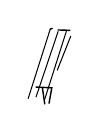
\begin{tikzpicture}[x=1mm,y=1mm,line cap=round]
\draw[line width=.13mm] (0,0)--(2.8,8.8) (1.0,.2)--(3.8,8.5) (2.1,-.1)--(4.9,8.7) (3.7,3.6)--(5.4,7.9);
\draw[line width=.18mm] (2.8,8.8)--(3.05,8.9) (3.8,8.7)--(5.3,8.65) (1.0,1.45)--(3.0,1.35)--(2.65,-.6) (1.8,1.4)--(2.1,-.7);
\end{tikzpicture}}

\margin{75}

\scanpage{75}
\[
\sum_1^n\log(1+r\rho_i(u+v))\leq\sum_1\log(1+r\rho_i(u))+\sum_1\log(1+r\rho_i(v))
\]

\[
S_{\deleted{\unsure{m}}\varphi}^{n}(u+v)\leq S_\varphi^n(u)+S_\varphi^n(v)\qquad S_\varphi^n(w)=\sum_1^n f_\varphi(\rho_i(w))
\]

\[
f_\varphi(\rho)=\int_0^{+\infty}\frac{\varphi(r)}{\frac1\rho+r}\,dr=\int_0^{+\infty}\varphi\left(\frac s\rho\right)\frac{ds}{1+s}
\]

$\varphi$ fonction décroissante

(motivation : \inserted{Si $A(0)=B(0)=0$ ($=0$ est un \unsure{symbole|exemple}), alors} $A(r)\leq B(r)$ pour $0\leq r\leq+\infty$ équivaut à $\int\psi(r)A(r)\,dr\leq\int\psi(r)B(r)\,dr$ pour toute $\psi\geq0$ à support cp\textsuperscript{t} dans $[a,b]$, Or, en posant $\psi(r)=-\varphi'(r)$, $\varphi$ fonction \unsure{décroissante} \inserted{\uline{continûment} \uline{différentiable}}, nulle en $b$ : \deleted{(\unsure{continûment}} \unsure{\deleted{\inserted{nulle}}|\inserted{nulle}} \deleted{\unsure{continue au} \illegible{1}} (ce qui est $+\infty$) et supposant \deleted{\unsure{de}}

que $A$ est dérivable $-\int\varphi'(r)A(r)\,dr=[-\varphi(r)A(r)]_0^{+\infty}+\int\varphi(r)A'(r)\,dr$ et le premier terme est nul, d'où $\int\varphi(r)A'(r)\,dr$. Si donc $A$ et $B$ sont dérivables, alors on obtient donc

\[
\int\varphi(r)A'(r)\,dr\leq\int\varphi(r)B'(r)\,dr
\]

pour toute fonction $\varphi$ continûment différentiable, décroissante \inserted{sur $[0,+\infty[$} et nulle au voisinage de $+\infty$. Si en plus $A'(r)$, $B'(r)\geq0$, alors ça sera vrai pour \deleted{toute} fonction décroissante \unsure{telle} ou nulle, pouvant être infinie. (Si on prend

$\varphi=$

\figure{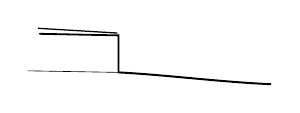
\begin{tikzpicture}[x=1mm,y=1mm,line cap=round]\draw[line width=.16mm] (0,5.6)--(10,5.0);\draw[line width=.23mm] (.2,4.9)--(10.2,4.7)--(10.2,0);\draw[line width=.08mm] (-1.3,.2)--(10.2,0);\draw[line width=.25mm] (10.2,0)..controls(16,-.3)and(23,-1.2)..(29.5,-1.5);\end{tikzpicture}}

, on retrouve $A(r)\leq B(r)$). Dans le cas actuel,

\[
A\deleted{\unsure{^{\,\prime}|{}^{\sim}}}(r)=\sum_1^n\log(1+r\rho_i(u))\qquad \text{donc }\ A'(r)=\sum\frac{r}{1+r\rho_i(u)}
\]

d'où notre assertion. -- Le cas le plus important est celui où on prend $\varphi(r)=r^{-p}$ $0<p<1$. On trouve alors

\margin{76}

\scanpage{76}
\[
f_\varphi(\rho)=\rho^p\int\frac{s^{-p}}{1+s}\,ds=c^{\mathrm{te}}.\rho^p,
\]

d'où, en posant \deleted{\unsure{Système|$S_p^{(n)}$}} a.

\[
S_p^{(n)}(u)=\sum_1^n\rho_i(u)^p
\]

\[
\boxed{S_p^{(n)}(u+v)\leq S_p^{(n)}(u)+S_p^{(n)}(v)}
\]

en particulier

\[
\boxed{S_p(u+v)\leq S_p(u)\unsure{-|+}S_p(v)}
\]

\reversemarginpar
\margin{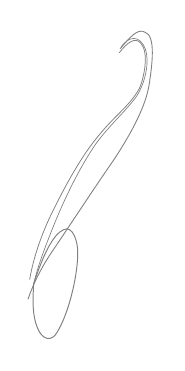
\begin{tikzpicture}[x=.1mm,y=-.1mm,line cap=round,line join=round,color=gray]
\draw[line width=.32pt] (138,33) .. controls (150,19) and (160,7) .. (169,12) .. controls (184,16) and (178,56) .. (175,77) .. controls (171,105) and (153,139) .. (130,174) .. controls (101,216) and (77,253) .. (52,290) .. controls (37,312) and (27,333) .. (21,351);
\draw[line width=.28pt] (137,38) .. controls (147,25) and (157,18) .. (164,26) .. controls (175,38) and (168,70) .. (163,82) .. controls (153,103) and (131,118) .. (111,143) .. controls (89,169) and (70,204) .. (53,238) .. controls (39,266) and (28,297) .. (23,326);
\draw[line width=.25pt] (139,31) .. controls (149,17) and (163,15) .. (170,34) .. controls (176,53) and (168,81) .. (157,96) .. controls (144,113) and (123,132) .. (107,154) .. controls (87,183) and (66,225) .. (49,269) .. controls (40,292) and (31,316) .. (27,337);
\draw[line width=.35pt] (28,332) .. controls (39,298) and (52,269) .. (66,263) .. controls (77,257) and (85,277) .. (84,296) .. controls (83,326) and (72,370) .. (58,393) .. controls (51,406) and (39,403) .. (33,388) .. controls (26,372) and (27,351) .. (28,332);
\end{tikzpicture}}
\normalmarginpar

\uline{Remarque} On a $\sum_1^n\rho_i(u+v)^p\leq\sum_1^n(\rho_i(u)^p+\rho_i(v)^p)$, quel que soit $n$, on peut donc appliquer le lemme de Weyl ; on trouve rien de spécial.

\uline{Question} Trouver la forme générale des fonctions $f$ d'une variable positive telle que, posant \deleted{\unsure{$S_f^{(n)}(u)$}} $f^{(n)}(u)=\sum_1^n\rho_i(u)$, on ait $f^{(n)}(u+v)\leq f^{(n)}(u)+f^{(n)}(v)$ quel que soit $n$. Il suffit qu'on ait $f^{\infty}(u+v)\leq f^{\infty}(u)+f^{\infty}(v)$

pour \uline{tout} $u\in L(E)$, avec $E$ espace de Hilbert de dimension finie arbitraire. Généralisation à des fonctions de $n$ arguments.

\figure{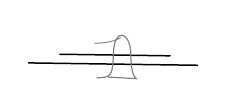
\begin{tikzpicture}[x=1mm,y=1mm,line cap=round]
\draw[line width=.19mm] (4,3)--(18,2.8) (0,1.9)--(21.5,1.6);
\draw[gray,line width=.15mm] (8.7,0).. controls (10.5,.1) and (10.7,.1)..(10.8,3.2)..controls (10.9,6.3) and (12.8,6)..(13,3.3)..controls (13,.8) and (13.4,.1)..(13.7,-.1)--(10.1,.1);
\draw[gray,line width=.12mm] (8.4,4.4)..controls (10.2,4.4) and (11.2,4.8)..(11.7,5.1);
\end{tikzpicture}}

\margin{77}

\scanpage{77}
/ op. hermitiens positifs, enfin satisfait à la formule (12).

\margin{\uline{Mettre en tête 2 et corollaire}}

\uline{Proposition 3} Soient $E$ et $F$ deux espaces de Hilbert, soient $u_i$ ($i=1,\mathord{.}\,\mathord{-}n$) des applications de Fredholm de $E$ dans $F$; alors $u_1\wedge\mathord{-}\wedge u_n$ est une application de Fredholm de $\overset{n}{\Lambda}^{(2)}E$ dans $\overset{n}{\Lambda}^{(2)}F$, et
\reversemarginpar\margin{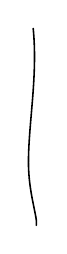
\begin{tikzpicture}[x=1mm,y=1mm,line cap=round]\draw[line width=.2mm] (.8,25) .. controls (1.4,19) and (.2,13) .. (.2,8) .. controls (.2,4) and (1.4,1) .. (1.2,0);\end{tikzpicture}}\normalmarginpar

\[
\begin{array}{@{}l@{\qquad}l@{}}
(13) & {\color{red}\boxed{\color{black}\displaystyle \lVert u_1\wedge\mathord{-}\wedge u_n\rVert_1\leq\frac1{n!}\lVert u_1\rVert_1\mathord{-}\lVert u_n\rVert_1}}
\end{array}
\]

En effet, il suffit de \deleted{\unsure{$\leq$}} vérifier \deleted{que si} si \deleted{$u_1=a_1'\otimes$} $u_i=\bar b_i\otimes a_i$, \deleted{\unsure{les} \illegible{1}} avec $\lVert\bar b_i\rVert\leq1$, $\lVert a_i\rVert\leq1$, alors $\lVert u_1\wedge\mathord{-}\wedge u_n\rVert_1\leq1/n!$, \deleted{\unsure{car}} puisqu'alors il existe une application \unsure{$n$ fois|de Ban} linéaire \deleted{\unsure{continue}} \inserted{de norme $\leq1/n!$} de $(\bar E\widehat{\otimes}E)^n$ dans \deleted{\unsure{dans}} $\bar F\widehat{\otimes}F$ (où $F=\overset{n}{\Lambda}^{(2)}E$) qui coïncide avec \inserted{$(u_1,\mathord{.}\,\mathord{-}u_n)\longrightarrow$} $u_1\wedge\mathord{-}\wedge u_n$ pour des $u_i$ décomposables, donc partout puisque les deux applications sont continues \deleted{\unsure{par}} en \deleted{\unsure{tant}} qu'applications, dans $L(F)$.

Or pour $u_i=\bar b_i\otimes a_i$, on a

\[
\deleted{\unsure{\overset{n}{\Lambda}}}\quad u_1\wedge\mathord{-}\wedge u_n=\frac1{n!}(\bar b_1\wedge\mathord{-}\wedge\bar b_n)\otimes(a_1\wedge\mathord{-}\wedge a_n),
\]

\inserted{(voir Chap I, N\textsuperscript{o} 1, formule (8))} d'où

\[
\lVert u_1\wedge\mathord{-}\wedge u_n\rVert_1\leq\frac1{n!}\lVert\bar b_1^c\wedge\mathord{-}\wedge\bar b_n\rVert\,\lVert a_1\wedge\mathord{-}\wedge a_n\rVert\leq\frac1{n!}\prod\lVert a_i\rVert\,\lVert\bar b_i\rVert
\]

(formule (5,), d'où (13).

\uline{Corollaire 1} Soit $E$ un espace de Hilbert, et \deleted{\unsure{$u$}}\inserted{$u,u_i$} $\in L^1(E;E)$ \inserted{$(i=1,\mathord{-} n)$} \deleted{des} opérateurs de Fredholm dans $E$. Alors $\overset{n}{\Lambda}u$ est un opérateur de Fredholm dans $\overset{n}{\Lambda}^{(2)}E$, et on a
\reversemarginpar\margin{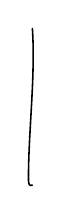
\begin{tikzpicture}[x=1mm,y=1mm,line cap=round]\draw[line width=.2mm] (.7,20) .. controls (1.1,14) and (.2,7) .. (.2,1) .. controls (.2,.1) and (.3,0) .. (.7,.1);\end{tikzpicture}}\normalmarginpar

\[
\begin{array}{@{}l@{\qquad}l@{\quad}l@{}}
(14) & \deleted{\unsure{\text{alors}}}\ \deleted{\unsure{\alpha_n(u)}}{\color{red}\boxed{\color{black}\displaystyle\left\{\begin{aligned}
\alpha_n u_1,\mathord{-}u_n)&=\operatorname{Tr}u_1\wedge\mathord{-}\wedge u_n)\\
\alpha_n(u)&=\operatorname{Tr}(\overset{n}{\Lambda}u)
\end{aligned}\right.}} & \begin{array}{@{}l@{}}\strut\\\text{en particulier}\end{array}
\end{array}
\]

(où $\alpha_n(u)$ est ${\color{red}\overline{\color{black}\text{défini dans}}}$ Chap 1, \S~2, prop 1) En effet, $(14)_{\unsure{2}}$ est vraie \deleted{pour \unsure{tout}} quand on

\margin{78}

\scanpage{78}
est de rang fini: \inserted{(vérifier d'après cas décomposable)} (voir Chap I, \S~1, N\textsuperscript{o} 2, définition 1), et reste donc vraie par raison de continuité dans le cas général. Conjointement avec (13), on trouve

{\reversemarginpar\margin{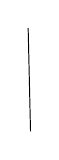
\begin{tikzpicture}[x=1cm,y=1cm]\draw[line width=.35pt] (0,0)--(.03,-1.31);\end{tikzpicture}}}
\uline{Corollaire 2} Sous les conditions précédentes, on a

\[
\begin{array}{@{}l@{\qquad}l@{}}
(15) & {\color{red}\boxed{{\color{black}\displaystyle |\alpha_n u_1,\mathord{-}u_n)|\leq\frac1{n!}\lVert u_1\rVert\mathord{-}\,\mathord{-}\lVert u_n\rVert}}}
\end{array}
\]

(Cela résulte aussi du fait, déjà signalé, que le coëfficient $k_n$ du Chap I, \S~1, N\textsuperscript{o} 2, prop 1, est ici égal à 1).

{\reversemarginpar\margin{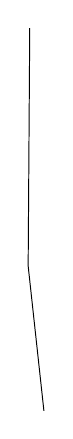
\begin{tikzpicture}[x=1cm,y=1cm]\draw[line width=.35pt] (0,0)--(-.02,-3.02)--(.18,-4.86);\end{tikzpicture}}}
\uline{Corollaire 3} Soit \deleted{$u\in L^1(E)$, où $E$ est un espace de Hilb} \inserted{$u$ un op. de Fredholm dans un} espace de Hilbert $E$. \deleted{Alors,} Si $u$ est un op. de Fredholm, il en est de même de $\overset{n}{\Lambda}u$, et on a

\[
\begin{array}{@{}l@{\qquad}l@{}}
(16) & \displaystyle \lVert\overset{n}{\Lambda}u\rVert_1=\alpha_n\deleted{\unsure{(\sqrt{u^*u})}}(|u|)\inserted{={\color{red}\underline{{\color{black}\alpha_n(\sqrt{\unsure{u^*u|u^*}})}}}}
\end{array}
\]

Si $u$ est un op. de H--S., il en est de même de $\overset{n}{\Lambda}u$, et on a

\[
\begin{array}{@{}l@{\qquad}l@{}}
(\unsure{17|14}) & \displaystyle \lVert\overset{n}{\Lambda}u\rVert_2=\sqrt{\alpha_n(u^*u)}
\end{array}
\]

On a, si $u\in L^1(E)$, $\lVert\overset{n}{\Lambda}u\rVert_1=\operatorname{Tr}\deleted{\sqrt{\vphantom{(\overset{n}{\Lambda}u)^*}}}\bigl((\overset{n}{\Lambda}u)^*(\overset{n}{\Lambda}u)\bigr)^{1/2}$ (N\textsuperscript{o} 1, formule (22)), or, (prop 1) on a $\deleted{\sqrt{\vphantom{(\overset{n}{\Lambda}u)^*}}}\bigl((\overset{n}{\Lambda}u)^*(\overset{n}{\Lambda}u)\bigr)^{1/2}=\overset{n}{\Lambda}\bigl((u^*u)^{1/2}\bigr)$, d'où \deleted{(16) en vertu de (17)} \inserted{$\lVert\overset{n}{\Lambda}u\rVert_1=\operatorname{Tr}\overset{n}{\Lambda}((u^*u)^{1/2})=\alpha_n(\sqrt{u^*u})$} (en vertu de (14)).

\deleted{Si $u\in L^2(E)$, \inserted{alors} on a encore, $(\overset{n}{\Lambda}u)^*(\overset{n}{\Lambda}u)=\overset{n}{\Lambda}(u^*u)$ \unsure{où on} \unsure{avait} $u^*u\in L^1(E)$ \inserted{est op. de Fredholm} (d'où $(\overset{n}{\Lambda}u)^*(\overset{n}{\Lambda}u)=\overset{n}{\Lambda}(u^*u)$ est $\in L^1(E)$, et $\overset{n}{\Lambda}u$ \unsure{par suite}}

Si $u$ est un op. de H.--S., alors $u^*u$ est un op. de Fredholm (N\textsuperscript{o} 1, th.~4), donc $(\overset{n}{\Lambda}u)^*(\overset{n}{\Lambda}u)=\overset{n}{\Lambda}(u^*u)$ est un op. de Fredholm, \deleted{et} donc $\overset{n}{\Lambda}u$ est un op. de H.--S. On a (N\textsuperscript{o} 1, th.~3, corollaire 3)

\[
(\lVert\overset{n}{\Lambda}u\rVert_2)^2=\operatorname{Tr}(\overset{n}{\Lambda}u)^*(\overset{n}{\Lambda}u)=\alpha_n(u^*u)\qquad\text{(formule (14), d'où (17))}
\]
{\reversemarginpar\margin{\unsure{79|75}}}

\cotefile{1}
\scanpage{79}

\reversemarginpar
\margin{\begin{tikzpicture}[x=1ex,y=1ex]
\draw[line width=.65pt] (.42,2.4) .. controls (.32,2.15) and (.33,1.95) .. (.53,1.82) -- (.57,.25) .. controls (.57,.05) and (.66,0) .. (.73,.04);
\draw[line width=.65pt] (.45,1.94) .. controls (.19,2.04) and (.12,1.91) .. (.15,1.67);
\end{tikzpicture}}
\normalmarginpar
\uline{Corollaire 4} Soit $u$ un op. de Fredholm dans l'espace de Hilbert $E$. Alors

\[
\text{(18)}\qquad {\color{red}\boxed{\color{black}|\alpha_n(u)|\leq\alpha_n(\deleted{\unsure{\sqrt{u^*u}}}|u|\deleted{{}_{\unsure{2}}})}}
\]

(\unsure{\deleted{En}|En} d'autres termes) les coefficients du développement de Fredholm $\det(1+zu)$ sont majorés en valeur, terme à terme, par les coefficients du déterminant de Fredholm $\det(1+z\unsure{h|H|\lvert u\rvert})$ relatif à l'hermitien positif $h=\sqrt{u^*u}$. On en conclut en effet

\uline{Corollaire 5} Dans les conditions précédentes, on a

\[
\text{(19)}\qquad |\det(1+zu)|\leq\det(1+|z|h)\quad\deleted{\unsure{(\det\sqrt{u^*u})}}
\]

\unsure{Montrons|Prouvons} (18). On a \inserted{en effet}, $|\alpha_nu|=|\mathrm{Tr}\,\overset{n}{\Lambda}u|\leq\|\overset{n}{\Lambda}u\|_1=\alpha_n(\sqrt{u^*u})$ (formule (16)).

\deleted{\uline{Théorème 2} Soit $u$ une \deleted{application}\inserted{op.} de Fredholm dans l'espace de Hilbert $H$. Alors la suite \inserted{$(\lambda_i)$} des valeurs propres \deleted{\illegible{1}} de $u$ est sommable \deleted{\unsure{et}} \deleted{\unsure{(1)|(19)}} \deleted{$\unsure{\sum_i|\lambda_i|\leq\lVert u\rVert_1}$} \deleted{\unsure{valeurs de $u$}}, on a}

\[
\text{\deleted{(20)}}\qquad {\color{red}\boxed{\color{black}\deleted{\det(1+u)=\prod_i(1+\lambda_i)}}}
\]

\deleted{\inserted{Appliquant (21) à $zu$ au lieu de $u$, on trouve}}

\deleted{\uline{Corollaire 1} Le déterminant de Fredholm de $\det(1+zu)$ de $u$ est une fonction entière de genre $0$\,;}

\[
\text{\deleted{(22)}}\qquad \deleted{\det(1+zu)=\prod_i(1+z\lambda_i)}
\]

\reversemarginpar
\margin{Le corollaire 1 ci-\unsure{$=$} équivaut \deleted{\unsure{aux}}\inserted{à la} formule,\par
$\text{(22)}\quad\alpha_n(u)=\sum_{i_1<\mathord{-}<i_n}\lambda_{i_1}\deleted{\unsure{(u)}}\mathord{-}\lambda_{i_n}\deleted{\unsure{(u)}}$\par
dont le plus intéressant est
\begin{tikzpicture}[x=1ex,y=1ex,baseline=0ex]
\draw[line width=.55pt] (.05,1.55) .. controls (.45,1.65) and (.66,1.83) .. (.91,1.99);
\draw[line width=.55pt] (1.45,1.39) -- (.58,.65) -- (.77,.52);
\end{tikzpicture}\par
$\text{(23)}\quad{\color{red}\boxed{\color{black}\mathrm{Tr}\,u=\sum\lambda_i(u)}}$}
\normalmarginpar

\deleted{\uline{Démonstration} du th. 2. \deleted{\unsure{Nous prouvons}} \unsure{On prouve d'abord le lemme} (20) \unsure{sur les valeurs}, \unsure{nous bornant à} la formule (20) : \unsure{soit un} \illegible{4}, \illegible{3} \unsure{propre}, \illegible{5}, \unsure{alors tout revient qu'il en est ainsi}, \unsure{et que} \illegible{1} \unsure{est identique dès que} \deleted{\unsure{tout}} \unsure{la} \illegible{1} \unsure{est nulle}.}

\margin{80}

\scanpage{81}

$f$ fonction convexe sur l'ouvert convexe $U$,

\[
(x,y)\in G_f\iff x\in U\text{ et } y>f(x)
\]

Soit \deleted{\unsure{$x_0,y_0$|$x,y$|$x_i,y_i$}} $(a,b)$ avec $b=f(a)$ $(a\in U)$, \deleted{\unsure{donc|on}} soit $H$ un hyperplan passant par $(a,b)$ ne rencontrant pas l'ouvert $G_f$, alors : 1) il est de la forme

\[
y-b=\deleted{\unsure{\sum c_i x_i+\beta}}=\sum c_i(x_i-a_i)
\]

(car ne contient pas la droite $x=a$), soit $y=L_a(x)$

2) On a $f(x)\geq L(x)$ pour \uline{\unsure{tout|tt}} $x\in U$ (en effet, l'un des deux \deleted{\unsure{hyperplans}} $\frac12$ espaces \inserted{ouverts} déterminés par $H$ contient $G_f$, et ce ne peut-être que celui donné par $y\geq L(x)$. \deleted{\unsure{donc}} d'où la conclusion), 3) On a pour $x\in E$ $f(x)=\sup_a L_a(x)$ (le sup étant obtenu), et réciproquement. 4) Si au point $a$, $f(x)$ est croissante alors les $c_i$ sont $\geq0$. En effet, si on avait p. ex $c_1<0$, alors $f(x_1,a_2,-a_n)$ est croissante au point $x_1=a_1$,
\reversemarginpar\margin{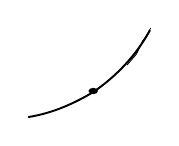
\begin{tikzpicture}[x=.1mm,y=-.1mm,line cap=round,line join=round]
\draw[line width=.7pt] (11,122) .. controls (42,117) and (68,105) .. (92,91) .. controls (122,71) and (148,43) .. (165,12);
\draw[line width=.25pt] (81,97) .. controls (105,84) and (129,63) .. (148,40) -- (166,9);
\draw[line width=.3pt] (136,56) -- (148,42) -- (156,25) -- (162,18);
\fill (93,89) ellipse (6 and 4);
\end{tikzpicture}}\normalmarginpar
et \deleted{de} minorée par $L(x_1,a_2-a_n)$, fonction linéaire prenant au \unsure{pt|point} $a$ la $=$ valeur que $f$. Cette dernière ne peut être strictement décroissante car on aurait $f(x_1)\leq f(a)\leq f(x_1)$ pour $x_1<a_1$ voisin de $a_1$.

\reversemarginpar\margin{82}\normalmarginpar

\scanpage{82}

§. \uline{Inégalités de convexité et degrés remarquables d'opérateurs, compacts}

\deleted{\unsure{La méthode de convexité}} \inserted{\textcircled{\scriptsize Th. 1}} \textcircled{1°} \deleted{\uline{Lemme fondamental}} \inserted{(H. Weyl).} Considérons deux suites finies
$(\alpha_i)_{1\leq i\leq n}$ et $(\beta_i)_{1\leq i\leq n}$ de nbs réels \inserted{on suppose} \deleted{la deuxième \unsure{décroissante}}

{\reversemarginpar\margin{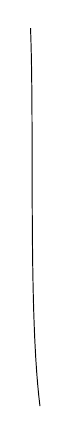
\begin{tikzpicture}[x=1cm,y=1cm]\draw[line width=.35pt] (0,0) .. controls (.05,-1.3) and (-.03,-3.6) .. (.12,-4.8);\end{tikzpicture}}}
\[
\begin{array}{@{}l@{\qquad}l@{}}
(1)&\displaystyle\boxed{\alpha_1\geq\alpha_2\mathord{.}\,\mathord{-}\,\mathord{-}\geq\alpha_n}\quad\text{et}\\
\text{\textcircled{2}}&\displaystyle\boxed{\boxed{\alpha_1+\mathord{-}\,\mathord{-}+\alpha_M\leq\beta_1+\mathord{-}+\beta_M\enspace\text{pour }M=1,\mathord{-}\,\mathord{-}n.}}
\end{array}
\]

Soit $\varphi(t_1,\mathord{-}\,\mathord{-}t_n)$ une fonction numérique \uline{convexe} et \uline{symétrique} sur $R^n$. On suppose vérifiée l'une des deux conditions suivantes : a) $\varphi$ est croissante \deleted{\unsure{(pour}}\inserted{en chaque argument $t_i$} \deleted{la \unsure{relation d'ordre naturelle|restriction d'un ensemble} sur $R^n$} b) $\sum_{i=1}^n\alpha_i=\sum_{i=1}^{n}\beta_i$.

{\reversemarginpar\margin{\begin{tikzpicture}[overlay,x=1cm,y=1cm]\draw[line width=.25pt] (.8,.2) .. controls (-.35,.4) and (-.35,-2.8) .. (.4,-3.1) .. controls (1.25,-3.5) and (2.1,-1.8) .. (1.9,-.1);\end{tikzpicture}\parbox[t]{1.85cm}{\unsure{fonction} où l'on \unsure{devrait} \unsure{admettre} \unsure{H} \illegible{1} \deleted{\unsure{partie}} \unsure{un} convexe ouvert.}}}

Sous ces conditions, on a
\[
\begin{array}{@{}l@{\qquad}l@{}}
(3)&\displaystyle\varphi(\alpha_1,\mathord{.}\,\mathord{-}\,\mathord{-},\alpha_n)\leq\varphi(\beta_1,\mathord{.}\,\mathord{-}\,\mathord{-}\beta_n)
\end{array}
\]

\deleted{Appliquons \unsure{tout de suite} le \unsure{corollaire|lemme} suivant, qui \inserted{\unsure{seul nous}} \illegible{1} \unsure{pour la} \unsure{question} qui \unsure{effacerait} \illegible{1}. On en conclut immédiatement le}

\deleted{\uline{Corollaire 1}} \inserted{\textcircled{\uuline{2°}}} Soit \inserted{$f(\rho_1,\mathord{-},\rho_n)$} fonction \deleted{\uline{\unsure{continue|numérique}}} \inserted{\uline{numérique symétrique}} de $n$ arguments \deleted{\unsure{positifs}} \inserted{$\rho_i>0$}, telle que $f(e^{t_1},\mathord{-}\,\mathord{-},e^{t_n})$ soit une fonction \uline{convexe} de $(t_1,\mathord{-}\,\mathord{-}t_n)\in R^n$. Soient $(\rho_1,\mathord{-}\rho_n)$ et $(\sigma_1,\mathord{-}\,\mathord{-},\sigma_n)$ deux suites \inserted{finies} positives, telles que \deleted{\unsure{(4bis)|(Hies.)}}

{\reversemarginpar\margin{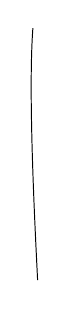
\begin{tikzpicture}[x=1cm,y=1cm]\draw[line width=.35pt] (0,0) .. controls (-.06,-.8) and (.02,-2.4) .. (.06,-3.2);\end{tikzpicture}}}
\[
\begin{array}{@{}l@{\qquad}l@{}}
\text{\textcircled{4}}&\displaystyle\boxed{\rho_1\geq\rho_2\mathord{-}\,\mathord{-}\geq\rho_n}\quad\text{et que }\deleted{\unsure{\sum\rho_i}}\\
\text{\textcircled{5}}&\displaystyle\boxed{\rho_1\mathord{.}\,\mathord{-}\rho_M\leq\sigma_1\mathord{.}\,\mathord{-}\sigma_M}\quad\text{pour }\deleted{\text{tout}}\ M=1,\mathord{-}n.
\end{array}
\]

On suppose vérifiée l'une des deux conditions suivantes :

{\reversemarginpar\margin{Il suffit que l'ensemble où est définie $f$ soit une partie \unsure{logarithmiquement} \unsure{convexe} \unsure{convenable} et symétrique.}}

a) $f$ est \inserted{définie et continue pour $\rho_i\geq0$, et} fonction croissante \deleted{des} \inserted{de} \deleted{\unsure{chacun des} $\rho_i$}\inserted{chaque argument $\unsure{\sigma_i|\rho_i}$} b) $\rho_1\mathord{.}\,\mathord{-}\rho_n=\sigma_1\mathord{-}\,\mathord{-}\sigma_n\ne0$. Sous ces conditions, on a
\[
\begin{array}{@{}l@{\qquad}l@{}}
\deleted{\unsure{(4)}}\ (6)&\displaystyle f(\rho_1,\mathord{-}\,\mathord{-}\rho_n)\leq f(\sigma_1,\mathord{.}\,\mathord{-}\sigma_n)
\end{array}
\]

En effet, si les $\rho_i,\sigma_i$ sont $>0$, cet énoncé est manifestement équivalent à l'énoncé du \deleted{lemme}\inserted{th.}, en posant $\alpha_i=\log\rho_i$, $\beta_i=\log\sigma_i$. \inserted{Cela prouve le \deleted{\unsure{corollaire}}\inserted{(2°)} en particulier dans le cas b).}

{\reversemarginpar\margin{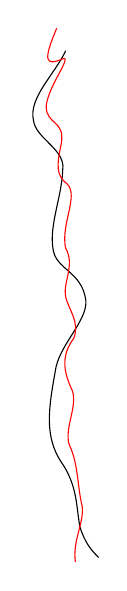
\begin{tikzpicture}[x=.0095cm,y=-.0095cm]
\draw[black] (65,37) .. controls (51,68) and (15,100) .. (22,130) .. controls (25,155) and (66,169) .. (61,197) .. controls (60,231) and (43,270) .. (48,301) .. controls (51,330) and (87,331) .. (92,371) .. controls (94,399) and (55,431) .. (51,466) .. controls (42,516) and (37,551) .. (58,585) .. controls (81,617) and (79,646) .. (84,673) .. controls (91,695) and (99,704) .. (109,714);
\draw[red] (53,7) .. controls (35,50) and (37,58) .. (61,48) .. controls (75,42) and (41,86) .. (39,111) .. controls (39,137) and (65,129) .. (59,162) .. controls (53,190) and (52,204) .. (67,215) .. controls (83,231) and (58,269) .. (65,301) .. controls (78,323) and (61,347) .. (65,366) .. controls (69,383) and (84,399) .. (76,421) .. controls (59,444) and (62,464) .. (72,487) .. controls (84,508) and (62,541) .. (70,564) .. controls (82,588) and (81,623) .. (87,645) .. controls (90,668) and (74,691) .. (78,720);
\end{tikzpicture}}}

\deleted{\unsure{On en conclut}, puisque} \inserted{Montrons que} \inserted{dans le cas a), tout} \deleted{l'ensemble des} systèmes $(\rho_i),(\sigma_i)$ tels que $\rho_i\geq0$, $\deleted{\unsure{\sigma_i\geq0|\rho_i>0}}$ \inserted{$\rho_1\geq\rho_2\mathord{-}\geq\rho_n\geq0$,} $\rho_1\mathord{.}\,\mathord{-}\mathord{.}\,\rho_M\leq\sigma_1\mathord{.}\,\mathord{-}\sigma_M$ pour $M=1,\mathord{-}\,\mathord{-}n$, \deleted{(et \unsure{éventuellement|naturellement} $\rho_1\mathord{.}\,\mathord{-}\rho_n=\sigma_1\mathord{-}\,\mathord{-}\sigma_n$)} \deleted{\unsure{est|et} l'adhérence} \inserted{est limite dans $R^{2n}$} de \deleted{sa partie formée des systèmes tels} \inserted{systèmes analogues} $(\rho'_i),(\sigma'_i)$ avec $\rho'_i>0$, $\sigma'_i>0$ (d'où résultera le \deleted{corollaire}\inserted{(2°) dans le cas a)} par prolongement par continuité). En effet, si \deleted{\unsure{les $\rho_i$}} \inserted{$\sigma_i>0$ pour tout $i$,} on voit qu'en \deleted{\unsure{tous les cas}} augmentant \inserted{de suffisamment peu} les $\rho_i$ qui seraient nuls, \deleted{\unsure{sont nuls, et il suffit d'approcher les systèmes}} on satisfait encore aux conditions imposées, \deleted{\unsure{et si} les systèmes $(\rho'_i),(\sigma'_i)$, avec $\rho'_i=\sigma'_i=\frac1n$ pour tout $i$. \unsure{D'autre part|diminuant}} d'où la conclusion \deleted{\unsure{voulue|cherchée}}\inserted{dans ce cas}.

{\reversemarginpar\margin{\unsure{{\color{red}?}}\kern-.3em\raisebox{-.7ex}{\unsure{{\color{black}?}}}}}

\deleted{Si plus généralement, \unsure{dans|donc} \illegible{1} \unsure{l'on} \illegible{2} \unsure{qui sont} \illegible{1} d'abord \illegible{1}}

{\reversemarginpar\margin{83}}

\scanpage{83}

\deleted{\unsure{approcher} $(\rho_i)(\sigma_i)$ par les systèmes $(\rho'_i)=(\unsure{\rho_i})$, $(\sigma_i+\varepsilon)$ \inserted{\deleted{$(\sigma'_i)=$}} \illegible{1} du \unsure{même} \illegible{1} \unsure{pour} $k=\unsure{n}$, $\rho'_i,\sigma'_i$ qui satisfont encore aux conditions \unsure{énumérées} \unsure{sauf} que $\sigma'_{n-1}\ne0$ (en \unsure{prenant|posant}}

Il suffit donc, dans le cas \deleted{\unsure{général}}\inserted{\unsure{$\sigma_n=0$|\deleted{$\sigma_n=0$}}}, \unsure{\deleted{d'approcher}|d'approcher|\deleted{d'associer}} \inserted{d'approcher} $(\rho_i)$ $(\sigma_i)$ par un \inserted{système admissible} $(\rho'_i),(\sigma'_i)$ avec $\sigma_n>0$, et on prendra \deleted{$\unsure{\rho'_i=\rho_i}$}

\deleted{\deleted{\unsure{évidemment}} \unsure{l'inégalité|simplement|supposons} par des $(\rho'_i),(\sigma'_i)$, avec $\sigma'_{n-1}>0$, comme on voit en posant $(\rho'_i)=(\rho_i)$, $\sigma_i=\sigma'_i+\varepsilon$ pour \deleted{tout} $i\leq n-1$, $\sigma'_n=\sigma_n$ (on aura un système admissible, en particulier $\prod\rho'_i=\prod\sigma'_i=0$), ce qui nous ramène au cas où $\unsure{\sigma}_{n-1}>0$, $\sigma_n=0$. \deleted{\unsure{et dont}}}

\deleted{Dans ce cas, si on prend $\sigma'_i=\sigma_i$ pour $i\leq n-1$, $\sigma'_n=\sigma_n+\varepsilon$, le système $(\rho_i),(\sigma'_i)$ est admissible, \inserted{pour $\varepsilon$ assez petit}, sauf que, dans le cas où on impose $\prod\rho_i=\prod\sigma_i$, on n'aura \deleted{\unsure{certainement|peut-être}} pas $\prod\rho_i=\prod\sigma'_i$. Mais en augmentant suffisamment peu les $\rho_i$ nuls, on obtient un système $(\rho'_i)$ tel qu'on ait encore \deleted{\unsure{et $\rho$}} $\rho'_1\mathord{-}\,\mathord{-}\rho'_q\leq\sigma'_1\mathord{-}\,\mathord{-}\sigma'_q$ pour $q=1,\mathord{-}n$, et \deleted{\unsure{même}}\inserted{par} augmentation éventuelle de $\rho'_n$ \deleted{\unsure{jusqu'à}}\inserted{$\rho''_n$}, \deleted{\unsure{on obtiendra|on obtient} $\rho'_1\mathord{.}\,\mathord{-}\rho'_{n-1}\rho''_n=\sigma'_1\mathord{-}\,\mathord{-}\sigma'_n$. \unsure{Ce système} $\rho'_n=$}}

simplement $\rho'_i=\rho_i$, $\sigma'_i=\sigma_i+\varepsilon$.

Prouvons maintenant le lemme. Il est bien connu qu'une \deleted{toute} fonction convexe \deleted{\unsure{$f$}} $\varphi$ sur $R^n$ est de la forme $\varphi=\operatorname*{Sup}_{\unsure{k|k\in K}}L_k$ où les $L_k$ sont des \deleted{\uline{\unsure{formes}}}\inserted{fonctions} \uline{linéaires} \inserted{affines} sur $R^n$ (\unsure{car|ça}. résulte du fait que la partie de $R^n\times R$ au dessus du graphe de $\varphi$ est convexe $\unsure{\div}$ par définition des fonctions convexes et \unsure{fermée|fermé} car $\varphi$ est continue, --- donc intersection de demi-espaces fermés, dont on constate aussitôt
\reversemarginpar
\margin{
\begin{tikzpicture}[x=1cm,y=1cm]\draw[red,line width=.55pt] (0.02,0.76) .. controls (-0.02,0.52) and (-0.02,0.20) .. (0.01,0);\end{tikzpicture}}
\normalmarginpar
qu'ils \deleted{\unsure{ne peuvent} \unsure{avoir} pour} \textcolor{red}{\uline{\textcolor{black}{\inserted{peuvent} se mettre}}} \textcolor{red}{\uline{\textcolor{black}{sous la forme}}} \inserted{d'équations} $L_k(t)\geq0$).

De plus, si $\varphi$ est croissante, on voit \deleted{\unsure{qu'on} \illegible{2}}\inserted{que} les $L_k$ crois\unsure{santes}, i.e. \deleted{à coefficients} de la forme $L_k(t)=\sum_{i=1}^n a_it_i+\unsure{h|b}$, \deleted{\unsure{où les}}\inserted{avec} $a_i\geq0$ \inserted{pour \deleted{tout} $i$}. \deleted{Pour le voir,} : En effet, si on avait $a_i<0$, alors \deleted{la fonction} on

\reversemarginpar
\margin{84}
\normalmarginpar

\scanpage{84}

fixant les arguments $t_j$ pour $j\ne i$, $L_k(t)=L_k(t_1,-t_n)$ \deleted{\unsure{devient|serait} \deleted{\illegible{1}} fonction linéaire strictement décroissante \deleted{\unsure{elle|$t_i$}} de $s=t_i$, majorée par la fonction continue croissante $\inserted{\varphi(\unsure{s|t})=}\varphi(t_1,-t_n)$, \deleted{\unsure{donc}} ce qui est manifestement impossible, \deleted{\unsure{puisque}}}\newline
\deleted{car $\unsure{\lambda_i|\lambda}$}\newline
\deleted{$\lambda(s)\to+\infty$ si $s\to-\infty$, et que $\varphi(s)$ reste borné pour $s\to-\infty$.}

on aurait $L(t)\to0$ si $t_i\to-\infty$, tandis que $\varphi(t)$ \deleted{\unsure{restant|resterait}}\inserted{resterait} borné pour $t_i\to-\infty$, ce \deleted{(\illegible{1} $\unsure{\varphi(t)}$} qui est incompatible avec $L(t)\leq\varphi(t)$ pour \deleted{tout} $t$. \deleted{\unsure{$f$}} Comme \deleted{\unsure{maintenant}}\inserted{enfin} $\varphi$ est aussi supposée symétrique, $L\deleted{\unsure{(t_1,-t_n)}}\leq\varphi\deleted{\unsure{(t_1,-t_n)}}$ \inserted{($L$ fonction sur $R^n$)} implique $\deleted{\unsure{L_k(t_{\sigma1},-t_{\sigma n})\leq\varphi(t_{\sigma1},\mathord{-}\,\mathord{-}t_{\sigma n})}}\inserted{\sigma L\leq\varphi}$ pour \deleted{tout} $\sigma\in\mathscr S_n$ (groupe des permutations des $n$ premiers entiers, i.e. \inserted{avec $\sigma L(t_1,-t_n)=L(t_{\sigma^{-1}1},\mathord{\cdot}\,\mathord{-}t_{\sigma^{-1}n})$}), donc on aura aussi

\[
\begin{array}{ll}
(7)&\displaystyle\deleted{\unsure{\varphi(t_1,-t_n)|\varphi(t)}}\varphi=\operatorname*{Sup}_k\operatorname*{Sup}_{\sigma\in\mathscr S_n}\sigma.L_k\deleted{\unsure{(t_1,-,t_n)}}
\end{array}
\]

Il s'ensuit que \deleted{\unsure{si}} pour prouver (1), il suffit de prouver que \inserted{pour $L\unsure{\in|=}L_k$, on a} \deleted{$\sigma L_k\deleted{\unsure{(\alpha_{\sigma1})}}\inserted{(\alpha_1,-\alpha_n)}\leq\varphi(\beta_1,-\beta_n)$ pour \deleted{tout} $k$, et tout $\sigma\in\mathscr S_n$. \unsure{Remplaçant|Remplaçons} \inserted{\deleted{\unsure{Désignant|Désignons}}} $L=$ $\sigma L_k$ par $L$, on est ramené à prouver}

\[
\begin{array}{ll}
(8)&\displaystyle\operatorname*{Sup}_{\sigma\in\mathscr S_n}(\sigma.L)(\alpha_1,\mathord{-}\,\mathord{\cdot}\alpha_n)\leq\operatorname*{Sup}_{\sigma\in\mathscr S_n}(\sigma L)(\beta_{\sigma1},\mathord{-}\,\mathord{-}\beta_{\unsure{\sigma n}})
\end{array}
\]

(car le deuxième mb en effet est $\leq\varphi(\beta_1,-\beta_n)$)\newline
\reversemarginpar\margin{\begin{tikzpicture}[x=1cm,y=1cm]\draw[red,line width=.4pt] (0,0)--(.02,.35);\end{tikzpicture}}\normalmarginpar
\begin{tikzpicture}[overlay,x=1cm,y=1cm]\draw[red,line width=.35pt] (0,-.22) .. controls (.45,-.38) and (.80,-.36) .. (1.25,-.28) .. controls (1.80,-.18) and (2.35,-.30) .. (2.90,-.29) .. controls (3.40,-.34) and (3.85,-.30) .. (4.20,-.24);\end{tikzpicture}
\deleted{\unsure{Pour le|Dans}}\inserted{Dans cette} inégalité, \deleted{\unsure{$L$ est une forme linéaire}} \inserted{$L(t_1,-t_n)=\sum_i^n a_it_i+b$}, \deleted{\unsure{affine et}} avec des \deleted{\unsure{$a_i$}} coefficients quelconques pour dans le cas b), et des $a_i>0$ pour tout $i$ dans le cas a) du lemme. \deleted{\inserted{\unsure{Désignons}} \unsure{Remarquons},} \inserted{On peut évidemment} \deleted{\unsure{résultat élémentaire} \unsure{bien} \illegible{1} \inserted{\unsure{Il suffit de démontrer que}}} supposer $b=0$.

\deleted{D'après un lemme connu, Il suffit \deleted{$\sum a_i\unsure{b_i}$} $L(\alpha_1,-,\alpha_n)\leq L(\quad$ \unsure{Notons que} $\sum a_i\alpha_i\leq\sum a_i\alpha_{\sigma i}$ quand $\sigma$ est une permutation telle que la suite des $a_{\sigma i}$ est \uline{décroissante}, ce qui}

D'après un lemme connu, \inserted{valable \unsure{donc puisque|du fait que} $\alpha_1\geq\alpha_2\geq-\geq\alpha_n$,} la somme $\sum a_{\sigma i}\alpha_i\inserted{=\sum a_i\alpha_{\sigma^{-1}i}}$ est maximum, pour $\sigma\in\mathscr S_n$ variable,

\reversemarginpar\margin{85}\normalmarginpar

\scanpage{85}

quand la suite $(a_{\sigma i})$ est décroissante, on est donc \deleted{\unsure{en changeant} au besoin \unsure{de notations}} \deleted{\unsure{supposer, pour prouver (8), que la suite} $a_1\geq a_2\mathord{-}\geq a_n$} ramené à prouver que si $a_1\geq a_2\mathord{-}\geq a_n$, on a $\sum a_i\alpha_i\leq\deleted{\unsure{a_i\alpha|a_i\alpha_i}}\sum a_i\beta_i\deleted{\sum a_i\unsure{\alpha|\alpha_i}}$, \deleted{\unsure{en supposant} \unsure{de plus}}\inserted{pourvu que} les $a_i$ soient positifs \deleted{si on n'est pas dans le cas b) du lemme} ou qu'on ait $\sum\alpha_i=\sum\beta_i$. Or on a en effet

\[
\begin{array}{@{}l@{\qquad}l@{}}
(9)&\displaystyle\sum a_i\unsure{\alpha|\beta}_i=(a_1-a_2)\unsure{\alpha|\beta}_1+(a_2-a_3)(\unsure{\alpha|\beta}_1+\unsure{\alpha|\beta}_2)+\mathord{-}+(a_{n-1}-a_n)(\unsure{\alpha|\beta}_1+\mathord{-}+\unsure{\alpha|\beta}_{n-1})\\
&\displaystyle\hfill+a_n(\unsure{\alpha|\beta}_1+\mathord{-}+\unsure{\alpha|\beta}_n)
\end{array}
\]

\deleted{\unsure{et on} $\leq$} et une formule analogue pour $\deleted{\sum a_i\unsure{\alpha_i}}\sum a_i\beta_i$. Comme les coefficients $(a_1-a_2)\mathord{.}\,\mathord{-}\,\mathord{-}(a_i-a_{i-1}),\mathord{-}\,\mathord{-}(a_{n-1}-a_n)$ sont positifs, \unsure{on} \deleted{\unsure{on conclut que la somme relative}} et que $\deleted{\sum}\alpha_1\leq\beta_1,\mathord{.}\,\mathord{-}\,\mathord{.}(\alpha_1+\mathord{-}+\alpha_{n-1})\leq(\beta_1+\mathord{-}+\beta_{n-1})$, on en conclut que tous les termes de la somme relative aux $\alpha_i$ sont majorés par les termes corres-\newline pondants de la somme relative aux $\beta_i$, à l'exception \inserted{à priori} du dernier. Mais on a aussi $a_n(\alpha_1\mathord{-}\alpha_n)\leq a_n(\beta_1+\mathord{-}\unsure{+}\beta_{\unsure{n|i}})$ dans \deleted{\unsure{du terme du dernier}}\inserted{le cas a)} du lemme ($a_n\geq0$, $\sum\alpha_i\leq\sum\beta$ et dans le cas b) ($\sum\alpha_i=\sum\beta_i$), d'où \deleted{la conclusion}\inserted{l'inégalité (1)}.

\deleted{\unsure{Notons}} Signalons en passant le

{\reversemarginpar\margin{\uline{petits caractères}}}
{\reversemarginpar\margin{\begin{tikzpicture}[x=.009cm,y=-.009cm]
\draw[line width=.35pt] (46,29) .. controls (56,42) and (54,88) .. (53,133) .. controls (52,192) and (47,231) .. (35,266) .. controls (23,303) and (21,350) .. (26,396) .. controls (30,448) and (45,496) .. (50,545) .. controls (56,594) and (46,639) .. (39,684) .. controls (28,741) and (26,781) .. (29,817) .. controls (31,837) and (38,852) .. (42,865);
\draw[line width=.45pt] (121,19) .. controls (122,58) and (109,104) .. (111,153) .. controls (112,176) and (115,203) .. (111,227);
\end{tikzpicture}}}

\uline{Corollaire \unsure{1a|bis|1bis}} Sous les conditions de \deleted{la prop. \unsure{du} \illegible{1}, b,} \deleted{\illegible{1}} \deleted{\unsure{corollaire 1}} \inserted{\uline{Th. 1, 2°, b)}} \deleted{\unsure{(resp. du corollaire 1, a))}} \deleted{la prop. \unsure{corollaire}, b)} on aura aussi, \deleted{\unsure{si on a pour tout} $\unsure{\sigma}$}

\[
\begin{array}{@{}l@{\qquad}l@{}}
(10)&\displaystyle f\left(\frac1{\sigma_1},\mathord{-}\,\mathord{-}\frac1{\sigma_n}\right)\leq f\left(\frac1{\rho_1},\mathord{-}\,\mathord{-},\frac1{\rho_n}\right)
\end{array}
\]

En effet, de $\rho_1\mathord{-}\rho_n=\sigma_1\mathord{-}\sigma_n$ on tire pour tout
{\reversemarginpar\margin{\inserted{$1\leq M\leq n$ :}}}

\[
\rho_M\rho_{M+1}\mathord{-}\rho_n=\frac{\sigma_1\mathord{-}\sigma_{M-1}}{\rho_1\mathord{-}\rho_{M-1}}\sigma_{\unsure{M}}\mathord{-}\,\mathord{-}\sigma_n,\qquad\text{d'où }\rho_M\mathord{-}\rho_n\leq\sigma_M\mathord{-}\,\mathord{-}\sigma_n
\]

en vertu de $\sigma_1\mathord{-}\sigma_{M-1}\leq\rho_1\mathord{-}\,\mathord{-}\rho_{M-1}$. Il s'ensuit que que les suites $(\frac1{\rho_n},\mathord{-}\frac1{\rho_1})$ et $((\frac1{\unsure{\rho_n|\sigma_n}},\mathord{.}\,\mathord{-}\frac1{\sigma_1})$ satisfont encore aux conditions du corollaire (la première étant décroissante, les produits \deleted{\unsure{qui interviennent par}} des $\frac1{\rho_i}$ ég. au produit des $\frac1{\sigma_i}$, et enfin $\frac1{\rho_n}\mathord{-}\,\mathord{-}\frac1{\rho_{\unsure{i}}}\leq\frac1{\sigma_{\unsure{n}}}\mathord{-}\,\mathord{-}\frac1{\sigma_{\unsure{i}}}$ pour $1\leq M\leq n$), d'où l'inégalité \unsure{(10)}.

{\reversemarginpar\margin{86}}

\scanpage{86}

\inserted{Bien entendu, on pourrait en \unsure{tirer} \unsure{analogues} \deleted{\illegible{1}} ad. lib}
\inserted{le Th. 1, 1°, hypothèse b)}

\deleted{Bien entendu, \unsure{en vertu de} l'inégalité \unsure{indiquée|analogue},}
\[
\deleted{(\unsure{7|4|11})\qquad \sum\varphi(-\alpha_1,\unsure{\mathord{-}},-\alpha_n)\leq\sum\varphi(\unsure{-}\beta_1,\unsure{\mathord{-}},\unsure{-}\beta_n)}
\]

\uline{Remarque 1} Notons, \deleted{\unsure{d'ailleurs|toutefois}}, que si deux suites $(\alpha_i)_{i\leq n},(\beta_i)_{i\leq n}$ satisfont aux conditions générales du \deleted{lemme}\inserted{th. 1, 1°} \inserted{$(\alpha_1\geq\mathord{-}\geq\alpha_n,\ \alpha_1+\unsure{\mathord{-}}\alpha_M\leq\beta_1+\mathord{\cdot}\,\mathord{\cdot}+\beta_M\ \deleted{\unsure{et}}\ 1\leq M\leq n$} alors \deleted{il en est de les \unsure{mêmes suites} $(\alpha_i)_{i\leq p},(\beta_i)_{i\leq p}$ pour tout $1\leq p\leq n$, \unsure{(pourvu bien entendu que} $\sum_1^p\alpha_i=\sum_1^p\beta_i$), donc on peut leur appliquer la \unsure{formule} du lemme, et \unsure{on obtient} par \unsure{exemple} $\varphi(\alpha_1,\unsure{\mathord{-}},\alpha_p)$ qu'on obtient en remplaçant $\alpha_{p+1},\unsure{\mathord{-}},\alpha_n$ et $\beta_{p+1},\unsure{\mathord{-}},\beta_n$ par}

\inserted{suites à $k$ éléments} $(\alpha_i)_{i\leq k}$ et $(\beta_i)_{i\leq k}$ \inserted{satisfont aux conditions analogues} \deleted{quelq que soit}\inserted{quel que soit} $1\leq k\leq n$. On peut donc appliquer à ces suites le $=$ lemme, et on trouve \deleted{\unsure{donc}}\inserted{p. ex.} que \deleted{\unsure{(quitte à} \illegible{2} \unsure{le lemme}} \inserted{si $\varphi$ est une fonction convexe} croissante de \uline{$k$} arguments, on a aussi $\varphi(\alpha_1,\mathord{\cdot}\,\mathord{-}\alpha_k)\leq\varphi(\beta_1,\mathord{-}\,\mathord{-},\beta_k)$. La remarque analogue vaut pour les \deleted{corollaire 1 du lemme}\inserted{conditions du th. 1, 2°}.

\reversemarginpar
\margin{\uline{Remarque 2} Si on suppose $(\alpha_i)$ $(\beta_i)$ \unsure{comme} dans l'hyp. a, et si $f(\alpha_1\mathord{-}\alpha_n)\leq f(\beta_1\mathord{-}\beta_n)$ pour \deleted{\unsure{toute}} $f$ \unsure{tel|telle} \unsure{$\in$|que} \ldots{} alors on a $\sum_1^m\alpha_i\leq\sum_1^m\beta_i$ (évidemment, cela revenant à $\sup_H\sum_{i\in H}\alpha_i$, \deleted{\unsure{où}} $H$ à \deleted{\unsure{au plus}} \inserted{$m$ éléments})}
\margin{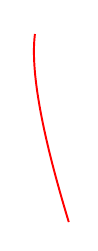
\begin{tikzpicture}[x=.01cm,y=-.01cm,baseline]\draw[red,line width=.7pt] (12,8) .. controls (4,70) and (35,181) .. (55,247);\end{tikzpicture}}
\normalmarginpar

\deleted{\uline{Applications \unsure{nouvelles de l'inégalité|et exemples de convexité} \unsure{au|du} corollaire 1.}}

Donnons maintenant un cas intéressant de fonctions $f$ satisfaisant aux conditions du \deleted{corollaire 1}\inserted{th. 1, 2°}. \deleted{\unsure{qui est}}

Si \uline{\deleted{\unsure{$f(\rho_1$}} $f(\rho_1,\mathord{-}\rho_n)$ est une fonction convexe croissante des \inserted{l'ens. des} arguments $\rho_i>0$, alors $f(e^{t_1},\mathord{-}e^{t_n})$ est \deleted{\unsure{convexe}}}\inserted{une} fonction convexe de \deleted{\unsure{chacun des arguments}} $(t_i)\in R^{n}$. Comme \deleted{la fonction convexe \unsure{sera celle qui est}} \inserted{$f$ sera} une enveloppe supérieure de fonctions \deleted{\unsure{linéaires}}\inserted{linéaires} affines \inserted{$\sum a_i x_i+\underset{\text{\unsure{qq}}}{b}$, $a_i\geq0$ (!)}, $f(e^{t_1},\mathord{-}e^{t_n})$ sera enveloppe supérieure \deleted{et que toute fonction convexe} de fonctions $\sum a_i e^{t_i}+b$, qui sont convexes (car \deleted{\unsure{si}} les fonctions $e^{t_i}$ sont convexes, et les $a_i$ positifs), donc elle sera elle-$=$ convexe.

En particulier, \deleted{si $f$ par une \deleted{fonction}\inserted{\unsure{norme}} de \unsure{Schatten}} \unsure{appelons|appl.ons}, \uline{\unsure{norme|normes} de Schatten} sur $R^n$ toute \uline{norme} $N(x)=N(x_1,\mathord{-}x_n)$ qui est symétrique, telle que $N(x_1,\mathord{-}x_n)=N(|x_1|,\mathord{-}\,\mathord{-}|x_n|)$, \deleted{et qui est fonction croissante de chacun des arguments pour} \inserted{$x_1\geq0,\mathord{-}\,\mathord{-}x_n\geq0$}, \deleted{\unsure{et par le fait est donc} \illegible{2}} \inserted{normalisée par $N(e_1)=1$.}

\reversemarginpar
\margin{
\begin{tikzpicture}[x=1cm,y=1cm,baseline]\draw[black!75,line width=1pt,line cap=round] (.02,.11)--(.27,.075)--(.53,.015);\draw[black!75,line width=.7pt,line cap=round] (.11,.025).. controls (-.015,.025) and (-.025,-.055)..(.16,-.035);\draw[red,line width=.65pt,line cap=round] (.025,.095)--(.50,.025);\draw[red,line width=.65pt,line cap=round] (.10,.055)--(.53,.01);\end{tikzpicture}}
\margin{(Alors on prouve que $N$ est fonction croissante \deleted{\unsure{des arguments}} \unsure{$(x_i)$|$(\alpha_i)$} dans \unsure{l'angle} des éléments positifs ((car la boule unité, étant stable par multiplication par une fonction $(\lambda_i)$ avec $|\lambda_i|=1$ pour \deleted{tout} $i$, le sera pour \deleted{\unsure{toute}} fonction majorée par $1$ en module).}
\margin{87}
\normalmarginpar

\scanpage{87}

\uline{norme de \unsure{Schatten}} $N(x_1,-x_n)$ \uline{satisfait \deleted{\unsure{à la|la}}\inserted{à \deleted{de} la} condition envisagée} \uline{dans l'énoncé du \deleted{corollaire 1}}\inserted{Th. 1, 2°} \deleted{\unsure{rappelé ci-dessus}}\inserted{pour la fonction $f$. On en conclut,} si $(\rho_i)$ \deleted{$\unsure{\rho(\sigma_i|\rho(x)}$} et $(\sigma_i)$ sont comme dans le th. :

\reversemarginpar
\margin{\textcircled{\unsure{11|13}} $N(\rho_1,-\rho_n)\leq N(\sigma_1,-\sigma_n)$ et plus généralement, compte tenu d'une remarque qui précède, et en \deleted{\unsure{pour que}} posant pour $1\leq k\leq n$ : $N(\rho_1,-\rho_k)=N(\rho_1,-\rho_k,0-0)$ \textcircled{12} $N(\rho_1,-\rho_k)\leq N(\sigma_1,-\sigma_k)$ pour $1\leq k\leq n$}
\normalmarginpar

\deleted{De =, \unsure{si on sait} que la fonction $(e^{t_i})^p$ étant une \unsure{fonction convexe}} \deleted{\inserted{\uline{la fonction} $f(r_1,-r_n)=r_1^p\unsure{-|+}+r_n^p$,} \uline{$p$ est un nb réel quelconque, satisfait aux \deleted{\unsure{conditions}}} \uline{conditions} \deleted{\unsure{du lemme}} \uline{envisagées dans le corollaire 1}, \deleted{\unsure{donc} \uline{dans l'hypothèse b, et = \deleted{\unsure{à toutes les}}\inserted{\unsure{on a|aux|cas a}} conditions envisagées} \uline{dans l'hypothèse a.}}}

Par suite, \deleted{\unsure{sous la condition,}}\inserted{sous les conditions} de l'hypothèse b, \deleted{\unsure{on}} $(\prod_1^M\rho_i\leq\prod_1^M\sigma_i\ \inserted{\text{pour }1\leq M\leq n},\ \prod_1\rho_i=\prod_1^n\sigma_i\ne0)$ on aura

\[
\begin{array}{ll}
(\unsure{1|9}5) & \displaystyle\sum_1^n\rho_i^p\leq\sum_1^n\sigma_i^p\qquad(p\text{ réel.})
\end{array}
\]

\deleted{\unsure{et dans le cas a|et sous les cond}} \inserted{et si $p\geq0$,} on aura, pourvu que $\prod_1^M\rho_i\leq\prod_1^M\sigma_i$ pour \inserted{$1\leq M\leq n$}, \deleted{on aura}

\[
\begin{array}{ll}
\deleted{\unsure{(12)}}\inserted{(16)} & \displaystyle\sum_1^k\rho_i^p\leq\sum_1^k\sigma_i^p\qquad(p\geq0,\ \deleted{\unsure{et}} k=1-n.)
\end{array}
\]

\deleted{Remarquons d'ailleurs que 2 \unsure{systèmes|suites} \inserted{\deleted{\unsure{positifs}}} $(\rho_i),(\sigma_i)$ \inserted{positifs} \unsure{donnés|formant}, \deleted{\unsure{dès}} satisfaisant aux inégalités (16), pour \deleted{tout} $k$, et \deleted{tout} $p$ \unsure{entier|réel} $\geq0$, on peut \uline{\unsure{propriété}} \unsure{réciproque|réciproquement}}

\deleted{\unsure{Nous pouvons arriver à}}

\reversemarginpar\margin{\uline{Th 2}}\normalmarginpar
(\uline{Premier Théorème de convexité dans les espaces de Hilbert})

\reversemarginpar
\margin{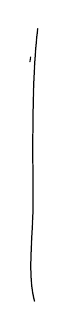
\begin{tikzpicture}[x=1cm,y=1cm]
\draw[line width=.45pt] (0,.02) .. controls (-.08,-.65) and (-.06,-1.5) .. (-.06,-2.3) .. controls (-.08,-2.8) and (-.12,-3.15) .. (-.04,-3.45);
\draw[line width=.4pt] (-.09,-.34)--(-.10,-.41);
\end{tikzpicture}}
\normalmarginpar
\deleted{\unsure{1)}} Soit $u$ un opérateur compact dans un espace de Hilbert, soit \deleted{$\varphi$ \unsure{la suite}} $f$\inserted{$(r_1,-r_n)$} une fonction \inserted{continue et symétrique} de $n$ arguments $r_i\geq0$, croissante \unsure{par r.|p. r.} à \unsure{chaq.|chaque} $r_i$, et telle que $f(e^{t_1},\mathord{-}\,\mathord{-},e^{t_n})$ soit fonction convexe de $(t_i)\in R^n$. Alors on a (\deleted{\unsure{en prenant} $\rho_i$} (avec les notations indiquées au N° \unsure{1|?|3}, avant la prop 3)

\[
\begin{array}{ll}
(17) & \displaystyle f(|\lambda_1|,\mathord{-}\,\mathord{-},|\lambda_n|)\leq f(\rho_1,\mathord{-}\,\mathord{-}\rho_n)
\end{array}
\]

Il suffit en effet de conjuguer le corollaire 1 du lemme 1 \deleted{\unsure{cas de}} (hypothèse a), avec le N° \unsure{?|1|2}, prop 3 ; corollaire 2. -- En particulier

\uline{Corollaire 1} Si $f\deleted{\unsure{(r)|(\rho)}}$ est une fonction \deleted{\unsure{croissante|convexe}}\inserted{continue} croissante de $r\geq0$ telle que $f(e^t)$ soit convexe, et $u$ un op. compact dans un espace de Hilbert, on a

\reversemarginpar\margin{88}\normalmarginpar

\scanpage{88}

En \unsure{dernier|deuxième} lieu, soit $f(s)$ une fonction définie pour $s>0$, telle que $f(e^t)$ soit convexe, posons $f(s_1,\mathord{-},s_n)=\sum_1^{\unsure{n}} f(s_i)$, c'est une fonction symétrique des \deleted{\unsure{nombres}}\inserted{\unsure{argts}} des $s_i>0$, et telle que $f(e^{t_1},\mathord{-}e^{t_n})$ soit convexe. Par suite, \deleted{\unsure{$F$}} $f(s_1,\unsure{\mathord{-}|\deleted{+}}s_n)$ satisfait aux conditions du corollaire 1, sous l'hypothèse b. Si on suppose de plus $f(s)$ croissante, et définie et continue aussi pour $s\geq0$, alors $f(s_1,\mathord{-}s_n)$ satisfait $=$ aux conditions du \deleted{corollaire 1}\inserted{\unsure{th.|Th.} 1, 2°} sous l'hypothèse a. D'où, \deleted{\unsure{avec la hypothèse}} \inserted{sous les conditions $\unsure{\rho_i>0}$,} \deleted{\unsure{convenables sur} $(\alpha_i),(\beta_i)$, \unsure{les inégalités}} l'inégalité

\[
\begin{array}{@{}l@{\qquad}l@{}}
(13)&\displaystyle \sum_1^n f(\rho_i)\leq\sum_1^n f(\sigma_i)
\end{array}
\]

et sous les conditions de b), compte tenu d'une remarque précédente, la suite d'inégalités

\[
\begin{array}{@{}l@{\qquad}l@{}}
(14)&\displaystyle \sum_1^k f(\rho_i)\leq\sum_1^k f(\sigma_i)\qquad(k=1,\mathord{-}n)
\end{array}
\]

Prenons p.ex, \deleted{\unsure{$p$ positif et}}\inserted{pour $p$ réel quelconque} $f(s)=s^p$, \inserted{$(s>0)$} on a alors $f(e^t)=e^{pt}$, qui est bien une fonction convexe. \deleted{\unsure{$f$ elle}}\inserted{$f(r)$} est définie et \deleted{\unsure{même}} continue pour $s\geq0$, et \deleted{\unsure{une}} fonction croissante de $s$, dès que $p\geq0$. \deleted{\unsure{les deux} \illegible{1}}

{\reversemarginpar\margin{89}}

\scanpage{89}

\reversemarginpar
\margin{$\unsure{k}$\par
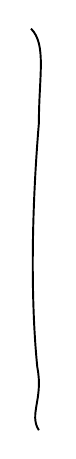
\begin{tikzpicture}[x=1mm,y=1mm,baseline=0pt]
\draw[line width=.7pt] (0,0) .. controls (2,-2) and (1,-6) .. (1,-12)
 .. controls (0,-24) and (0,-35) .. (.8,-43)
 .. controls (1.6,-47) and (-.3,-49) .. (1,-51);
\end{tikzpicture}}
\normalmarginpar

\[
\begin{array}{ll}
(18)&\displaystyle
\deleted{\unsure{f(\rho|f(\rho)}}
\sum_1^{\unsure{n|k}}f(|\lambda_i|)\leq\sum_1^k f(\rho_i)
\qquad
\overset{\inserted{(k:1,\ldots)}}{\deleted{(k\leq\dim\unsure{H|E})}}
\end{array}
\]

En particulier, \deleted{\unsure{pour que}} si
\deleted{\unsure{$\dim$}}\inserted{$E$} est de dimension infinie,
si \inserted{la série} $\sum_{i=0}^{\infty}f(\rho_i)$
\deleted{\unsure{conv., alors|conv, alors|converge, alors}}\inserted{est convergente},
il en est de $=$ de
$\sum_{\unsure{j|i}\unsure{\geq|=}0}^{\unsure{-\infty|\infty}}f(|\lambda_i|)$, et on a

\[
\begin{array}{ll}
(19)&\displaystyle\sum_{i=1}^{\infty}f(|\lambda_i|)\leq\sum_{i=0}^{\infty}f(\rho_i)
\end{array}
\]

En particulier, faisant $f(\unsure{a|r})=r^p$ $(p>0)$, on tir\unsure{e}

\uline{Corollaire 2} Soit $u$ un op. compact dans un espace de
\reversemarginpar
\margin{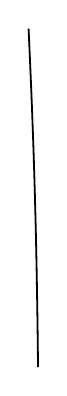
\begin{tikzpicture}[x=1mm,y=1mm,baseline=0pt]
\draw[line width=.65pt] (0,0) .. controls (.5,-11) and (1,-23) .. (1.2,-43);
\end{tikzpicture}}
\normalmarginpar
Hilbert $E$, et soit $p>0$. Alors, pour tout entier $k>0$

\[
\begingroup
\setbox0=\hbox{$\displaystyle\sum_{i=1}^k|\lambda_i|^p\leq\sum_{\unsure{j|i}=1}^k\rho_i^p=$}
\setbox2=\hbox{$\displaystyle\deleted{\|u\|_p}$}
\begin{array}{ll}
(20)&
\smash{\rlap{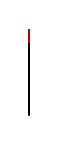
\begin{tikzpicture}[x=\wd0,y=1ex,baseline=0pt]
\draw[red!75!black,line width=1pt] (-.025,-3.2)--(-.02,3.4)--(1.09,3.9);
\draw[red!75!black,line width=1pt] (1.02,3.0)--(1.025,-3.15)--(-.025,-3.2);
\draw[red!75!black,line width=.8pt] (-.025,-3.35) .. controls (.35,-3.35) and (.8,-3.0) .. (1.025,-2.95);
\draw[line width=.6pt] (.025,2.7)--(-.07,1.6)--(.025,2.3)--(-.07,-.3)
 --(.04,.3)--(-.03,-3.3)--(.19,-1.75)--(.08,-3.3)--(.48,-1.5)
 --(.39,-3.2)--(.65,-1.4)--(.61,-2.7)
 .. controls (.79,-2.2) and (.93,-2.25) .. (.97,-2.5);
\end{tikzpicture}}}\box0\hspace{.5em}
\smash{\rlap{\begin{tikzpicture}[x=\wd2,y=1ex,baseline=0pt]
\draw[line width=.6pt] (-.1,3.5)--(1.14,3.4)--(1.18,-2.55);
\draw[line width=.6pt] (1.0,-2.5) .. controls (.5,-2.9) and (.05,-2.85) .. (-.2,-2.5);
\draw[line width=.7pt] (.1,3.45)--(-.22,1.7)--(.42,3.35)--(-.08,.8)--(.57,2.0)--(.1,-.1)--(.98,-.25);
\end{tikzpicture}}}\box2
\qquad
\setbox4=\hbox{$\deleted{(k\leq\dim\unsure{H|E})}$}
\smash{\rlap{\begin{tikzpicture}[x=\wd4,y=1ex,baseline=0pt]
\draw[line width=.6pt] (.01,1.85)--(.095,1.5)--(.205,2.7)--(.145,.95)--(.36,2.55)--(.28,.55)--(.55,1.95)--(.47,.5)--(.92,1.35);
\end{tikzpicture}}}\box4
\end{array}
\endgroup
\]

\deleted{\unsure{en particulier}, si $E$ est de dimension finie $n$}

\[
\begingroup
\setbox0=\hbox{$\displaystyle\sum_i|\lambda_i|^p\leq\sum_i\rho_i^p=\|u\|_p$}
\begin{array}{ll}
(21)&\smash{\rlap{\begin{tikzpicture}[x=\wd0,y=1ex,baseline=0pt]
\draw[red!75!black,line width=1pt] (-.03,3.45)--(-.025,-2.9)
 .. controls (.4,-2.85) and (.8,-2.6) .. (1.035,-2.55);
\draw[red!75!black,line width=1pt] (1.055,2.6)--(1.05,-2.25);
\draw[red!75!black,line width=1pt] (-.02,3.55) .. controls (.4,3.8) and (.75,3.8) .. (1.07,3.5);
\end{tikzpicture}}}\box0
\end{array}
\endgroup
\]

(où la somme est prise sur tous les indices $i$) En particulier, faisant $p=1$ et $p=2$,
et \unsure{appliquant|utilisant} le N° 1, th. 2 et th. 3, formules (15) et (20), on trouve

\uline{Corollaire 3} Soit $u$ un op. \deleted{\unsure{dont}} de Fredholm
(resp\textsuperscript{t} un op. de \deleted{\unsure{Hilb|Hilb.}} H.-S.) dans
\deleted{l'\unsure{espace|aire}}\inserted{un espace} de Hilbert.
\deleted{\unsure{Et,|Et}} Alors \deleted{\unsure{une}} la suite des valeurs propres
est sommable (resp\textsuperscript{t}. de carré sommable) et on a

\[
\begingroup
\setbox0=\hbox{$\displaystyle\sum|\lambda_i|\leq\|u\|_1$}
\setbox2=\hbox{$\displaystyle\left(\sum|\lambda_i|^2\right)^{1/2}\leq\|u\|_2$}
\begin{array}{ll}
(21)&\smash{\rlap{\begin{tikzpicture}[x=\wd2,y=1ex,baseline=0pt]
\draw[red!75!black,line width=1pt] (-.03,2.8)--(-.05,-1.8)--(.98,-1.7)--(.995,2.55);
\draw[red!75!black,line width=1pt] (.1,3.0) .. controls (.4,3.3) and (.7,3.2) .. (1.07,2.95);
\end{tikzpicture}}}\hbox to\wd2{\box0\hfil}\\[2.7ex]
(22)&\smash{\rlap{\begin{tikzpicture}[x=\wd2,y=1ex,baseline=0pt]
\draw[red!75!black,line width=1pt] (-.05,3.4) .. controls (.25,3.25) and (.75,3.6) .. (1.03,3.45);
\draw[red!75!black,line width=1pt] (-.065,2.8)--(-.065,-2.45)
 .. controls (-.06,-2.85) and (-.04,-2.95) .. (0,-2.9)--(1.04,-2.55);
\draw[red!75!black,line width=1pt] (1.055,2.8)--(1.07,-2.7);
\end{tikzpicture}}}\box2
\end{array}
\endgroup
\]

Signalons aussi le

\uline{Corollaire 4} Soit $u$ un op. \deleted{\unsure{dans}}\inserted{lin.} dans un espace
\reversemarginpar
\margin{\shortstack[l]{petits\\caractères}\par
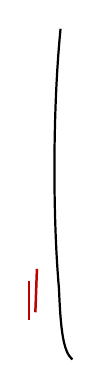
\begin{tikzpicture}[x=1mm,y=1mm,baseline=0pt]
\draw[line width=.8pt] (1,0) .. controls (0,-10) and (0,-24) .. (.8,-33)
 .. controls (1,-38) and (1.3,-41) .. (2.5,-42);
\draw[red!75!black,line width=1pt] (-3,-32)--(-3,-37);
\draw[red!75!black,line width=.9pt] (-2,-30.5)--(-2.2,-36);
\end{tikzpicture}}
\normalmarginpar
de Hilbert de dimension finie $n$, \deleted{Alors,} soit
$f(s_1,\mathord{-}s_n)$ \deleted{\unsure{est}} une fonction de \inserted{$n$} arguments $s_i>0$
telle que $f(e^{t_1},\mathord{-}e^{t_n})$ soit convexe (pas forcément croissante).
Si $f$ est en fait définie et continue pour \deleted{\unsure{les}} $s_i\geq0$,
ou si $u$ est inversible, on a

\[
\begingroup
\setbox0=\hbox{$\displaystyle f(|\lambda_1|,\mathord{-}|\lambda_n|)\leq f(\rho_1,\mathord{-},\rho_n)$}
\begin{array}{ll}
\text{\textcircled{23}}&
\smash{\rlap{\begin{tikzpicture}[x=\wd0,y=1ex,baseline=0pt]
\draw[line width=.65pt] (.13,3.45) .. controls (.4,3.1) and (.75,3.6) .. (1.02,3.55);
\draw[line width=.75pt] (-.025,2.85)--(-.025,-1.55)
 .. controls (-.02,-2.1) and (.02,-2.25) .. (.08,-2.15)
 .. controls (.42,-1.7) and (.78,-1.75) .. (1.015,-1.75);
\end{tikzpicture}}}\box0\unsure{!|.}
\end{array}
\endgroup
\]

\deleted{\unsure{(23)|Alors}} En effet, on a, en plus des inégalités
$|\lambda_1\mathord{-}\lambda_n|\leq\rho_1\mathord{-}\rho_n$ $(k\leq n)$, l'\uline{égalité}

\reversemarginpar\margin{90}\normalmarginpar

\scanpage{90}

\[
\text{(24)}\qquad |\lambda_1|\mathord{-}|\lambda_n|=\rho_1\mathord{-}\rho_n
\]

\deleted{En effet, le \deleted{\unsure{produit}}\inserted{carré du premier} mb est égal à \deleted{$|\lambda_1\unsure{\rho|q}$} $|\lambda_1\mathord{\cdot}\,\mathord{-}\lambda_n|^2=|\det u|^2=(\overline{\det u},\unsure{\overset{\deleted{\mathrm{conj}}}{\det u}|\overline{\det u}})=(\det u^*)\det u\deleted{{}^{\unsure{*}}}=\det u^*u=\rho_1^2\mathord{-}\,\mathord{-}\rho_n^2$, où $\rho_1\mathord{-}\rho_n$ sont les valeurs propres de $(u^*u)^{1/2}$, d'où (23).}
\textcolor{red}{\uline{\textcolor{black}{Il \deleted{\unsure{que}} \inserted{\deleted{\unsure{d'où}}} s'ensuit, \unsure{ainsi|alors},}}}

\reversemarginpar
\margin{On a \deleted{\unsure{d'autre|d'une part} $\unsure{\lambda_1}\mathord{-}\lambda_n=\det\inserted{\deleted{\unsure{u}}}$}
\begingroup\setbox0=\hbox{$\text{(25)}\quad\lambda_1(u)\mathord{-}\lambda_n(u)=\det u$}\dimen0=\wd0\advance\dimen0 by6pt\dimen2=\ht0\advance\dimen2 by3pt\dimen4=\dp0\advance\dimen4 by3pt\dimen6=\dimen4\advance\dimen6 by-2pt\leavevmode\hspace{3pt}\rlap{\begin{tikzpicture}[overlay,baseline=0pt]\draw[line width=.45pt] (-3pt,\the\dimen2)--(-3pt,-\the\dimen4)--(\the\wd0,-\the\dimen4);\draw[line width=.45pt] (\the\dimen0,-\the\dimen6)--(\the\dimen0,\the\dimen2);\end{tikzpicture}}\box0\hspace{6pt}\endgroup
\deleted{et de} d'autre part $(\rho_1(u)\mathord{-}\rho_n(u))^2=\rho_1(u^*u)\mathord{\cdot}\,\mathord{-}\rho_n(u^*u)=\det(u^*u)=\det u^*\,\det u=\overline{\det u}\det u=|\det u|^2$, d'où
\begingroup\setbox0=\hbox{$\deleted{\unsure{(25)|(24)}}\ \text{\textcircled{26}}\quad\rho_1(u)\mathord{-}\rho_n(u)=\det|u|$}\dimen0=\wd0\advance\dimen0 by3pt\dimen2=\ht0\advance\dimen2 by3pt\dimen4=\dp0\advance\dimen4 by3pt\dimen6=\wd0\divide\dimen6 by10\dimen8=\wd0\advance\dimen8 by-\dimen6\dimen6=\dimen4\advance\dimen6 by-2pt\leavevmode\hspace{3pt}\rlap{\begin{tikzpicture}[overlay,baseline=0pt]\draw[line width=.45pt] (0pt,\the\dimen2)--(\the\dimen0,\the\dimen2);\draw[line width=.45pt] (-3pt,\the\dimen2)--(-3pt,-\the\dimen4)--(\the\dimen0,-\the\dimen4);\draw[line width=.45pt] (\the\dimen8,-\the\dimen4) to[out=70,in=180] (\the\wd0,-\the\dimen6);\end{tikzpicture}}\box0\hspace{3pt}\endgroup
En comparant (25) et (26), \unsure{tr.|t.} $\Rightarrow$ (24)}
\normalmarginpar

quand $u$ est inversible, \deleted{que} donc \deleted{$|\lambda_1\mathord{-}\lambda_n|$ \unsure{et}} les $\lambda_i$ et les $\rho_i$ non nuls \deleted{\unsure{que ce sont}}, que les conditions du \deleted{corollaire 1 du lemme fondamental 2 sont vérifiées, dans l'hypothèse b)} \inserted{\unsure{th.|Pr.} 1, 2\uuline{°}, hypo. b sont vérifiées.} Si on suppose que $f$ est de plus \textcolor{red}{\uline{\textcolor{black}{définie}}} et continue pour $r_i\geq0$, comme on aura (23) pour \deleted{tout} $u$ inversible et que les deux mbs sont des fonctions continues de $u$ comme on vérifie aussitôt, il s'ensuit que l'inégalité sera vérifiée pour \deleted{tout} $u$. -- Le

\deleted{\uline{Corollaire 5}} résulte p. ex du corollaire 4 que si $u$ est inversible, les formules (21) sont vérifiées $=$ si $p$ n'est pas positif. Notons que \deleted{sous les conditions du corollaire 3, on tire de \unsure{(24)|(26)} et des inégalités $|\lambda_1\mathord{-}\lambda_k|\leq\rho_1\mathord{-}\rho_k$, \unsure{les relations analogues}}

\reversemarginpar
\margin{\deleted{\unsure{(25)|(24)|(27)} $|\lambda_k\mathord{-}\lambda_n|\leq\rho_{\unsure{k|n}}\mathord{-}\rho_n$ $(1\leq k\leq n)$, \unsure{ce qui} \illegible{2} pour $\unsure{\rho_k}\mathord{-}\unsure{\rho_n}$, \illegible{3} \unsure{la} \illegible{2}} \textcolor{red}{\textcircled{?}}}
\margin{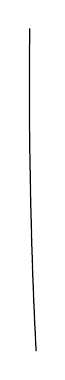
\begin{tikzpicture}[x=1cm,y=1cm]\draw[line width=.45pt] (0,0) .. controls (-.02,-1.05) and (.01,-2.85) .. (.08,-4.1);\end{tikzpicture}}
\normalmarginpar

\uline{Corollaire 5} Soit $u$ un opérateur dans un espace de Hilbert $E$, soit $N$ une norme de Schatten sur $R^{\deleted{I}\inserted{k}}$, \deleted{où $I=\deleted{\dim}(1,\unsure{\mathord{-}}n)$ \unsure{si} $\dim E=n$, et $I=$ ensemble des entiers si} \inserted{où $k\leq\dim E$.} \inserted{Alors, on a}

\[
\text{(27)}\qquad N(|\lambda_1|,\mathord{-}\,\mathord{-}|\lambda_k|)\leq N(\rho_1,\mathord{-}\,\mathord{-}\rho_k)
\]

\deleted{D'où, $\unsure{N(}\unsure{\leq|\xi|k|\lambda_i}$} Par suite, si la dimension de $E$ est infinie et si $N$ est une norme de Schatten sur \deleted{\unsure{tout|de}} l'espace $R^{(\underline N)}$, \deleted{\unsure{lorsque} $\underline N$ \unsure{désigne}} \inserted{on a}

\[
\text{\unsure{(28)|(26)}}\qquad N((|\lambda_i|))\leq N((\rho_i))
\]

Dans cet énoncé, $\underline N$ désigne l'ensemble des entiers, donc $R^{(\underline N)}$ l'espace des suites de \unsure{nbs réels|nbs entrs} \deleted{\unsure{qui sont}} dont seul un nb fini de termes sont non nuls. Une norme sur $R^{(\underline N)}$ est dite une norme de Schatten, si elle induit une norme de Schatten sur \deleted{tout} un, espace $R^n$ (plongé de façon naturelle dans $R^{(\underline N)}$).

\reversemarginpar
\margin{91}
\normalmarginpar

\scanpage{91}

\deleted{\unsure{La formule}} Enfin, si $\xi=(\xi_i)$ est une suite quelconque de nbs réels \deleted{positifs}, posons $x_n=(\unsure{\xi_1|\xi'_1}\mathord{-}\xi_n,0,\mathord{-}0)$, alors $N(x_n)$ \deleted{a une limite \unsure{quand} \illegible{1} de $n$}, \inserted{croît avec $n$, et} on pose $N(\xi)=N((\xi_i))=\lim_n N(x_n)$, nb fini ou infini. $\geq0$

\deleted{\unsure{Ainsi|Alors}} La formule (25) est un cas particulier du théorème, car $N$ \deleted{\unsure{jouit des pp.}}\inserted{satisfait aux} conditions envisagées pour $f$ dans cet énoncé. La formule (26) en résulte par un passage à la limite.

{\reversemarginpar\margin{\uline{Th 3}}}\uline{Deuxième théorème de convexité dans les espaces de Hilbert}

{\reversemarginpar\margin{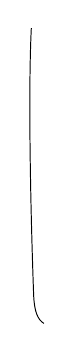
\begin{tikzpicture}[x=1cm,y=1cm]\draw[line width=.35pt] (0,0) .. controls (-.04,-.8) and (-.01,-2.3) .. (.03,-3.4) .. controls (.04,-3.6) and (.08,-3.7) .. (.16,-3.75);\end{tikzpicture}}}
Soi\deleted{\unsure{ent}}\inserted{\unsure{nt|ent}} $E,F,\unsure{C|G}$ trois espaces de Hilbert, soit $u$ une application linéaire \deleted{continue}\inserted{cpt} de $E$ dans $F$, \deleted{$E$} $v$ une application linéaire \deleted{continue}\inserted{cpt} de $F$ dans $\unsure{C|G}$, \deleted{soit $\unsure{u|n}$ un entier positif} enfin soit $f(s_1,\mathord{-}s_n)$ une fonction continue \inserted{symétrique et croissante} de $n$ arguments $s_i\geq0$, telle que \deleted{la fonction} $f(e^{t_1},\mathord{-},e^{t_n})$ soit fonction convexe de $(t_i)\in R^n$. Alors on a

\[
\begin{array}{@{}l@{\qquad}l@{}}
(29)&\displaystyle f(\rho_1(uv),\mathord{-}\rho_n(uv))\leq f(\rho_1(u)\rho_1(v),\mathord{\cdot}\,\mathord{-},\rho_n(u)\rho_n(v)\unsure{,})
\end{array}
\]

En effet, il suffit de \deleted{conjuguer}\inserted{\unsure{l'appliquer|appliquer}} le \deleted{lemme}\inserted{th. 1} \deleted{fondamental, \unsure{corollaire} 1, \unsure{condition}} aux deux suites $(\rho_i(uv))_{i\leq n}$ et $(\rho_i(u)\rho_i(v))_{i=n}$. Les conditions \inserted{a l'hyp. b n° 2°) du th 1.} du \deleted{corollaire 1 de ce lemme} sont satisfaites, \deleted{\unsure{en ef}} en vertu du N° \unsure{?|7}, prop. 2, corollaire 3. \deleted{(\unsure{en effet} \illegible{1})}.

\uline{Corollaire 1} Soient $u$ et $v$ \deleted{comme} dans le th. 3, soit $f(r)$ une fonction continue croissante de $r\geq0$ telle que $f(e^t)$ soit fonction convexe de $t\in R$. Alors, pour \deleted{tout \unsure{nbre}} entier $n>0$, on a

{\reversemarginpar\margin{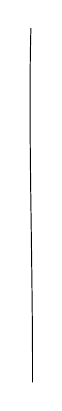
\begin{tikzpicture}[x=1cm,y=1cm]\draw[line width=.35pt] (0,0) .. controls (-.035,-1.25) and (.025,-3) .. (.02,-4.5);\end{tikzpicture}}}
{\reversemarginpar\margin{\illegible{1} $\unsure{l}$\\\deleted{\illegible{1}}\\\deleted{\illegible{1}}\\\deleted{\illegible{1}}}}
\[
\begin{array}{@{}l@{\qquad}l@{}}
(30)&\displaystyle \sum_{i=1}^n f(\rho_i(uv))\leq\sum_{i=1}^n f(\rho_i(u)\rho_i(v))
\end{array}
\]

\deleted{d'où} \inserted{d'où}

\[
\begin{array}{@{}l@{\qquad}l@{}}
(3\unsure{1|4})&\displaystyle \sum_{\unsure{j|i}} f(\rho_i(uv))\leq\sum_{i\unsure{\mathord{-}|=}} f(\rho_i(u)\rho_i(v))
\end{array}
\]

(les sommes étant étendues à tous les indices $i$.)

\deleted{\illegible{1} $\unsure{(\rho_i(uv))|(\rho_i(vu))}$ \unsure{associée} \illegible{2} \unsure{des suites} $(\rho_i(u))$}

\deleted{$(\rho_i(v))$ associée à $u$ resp. $v$, \unsure{les|la} $=$s \unsure{majoration|majorations} \deleted{\unsure{pour tout}} que celle qui vaudrait si on avait $\unsure{\cdot}uv)=\rho_i(u)\rho_i(v)$, donc si $u$ et $v$ étaient des \unsure{p}érateurs de multiplication dans $l^{\unsure{?|2}}$ par les \unsure{tes} $(\rho_i(u))$ resp.\textsuperscript{t} $(\rho_i(v))$. \deleted{\unsure{En particularisant}} \inserted{\uline{Mais} \unsure{prévoir|pourquoi|pourrait} aussi.} \deleted{\unsure{ce dernier, il}} donner un corollaire \deleted{qui} analogue \deleted{\uline{\unsure{Théorème 4}} \unsure{Soient}} au corollaire 4 du th. 1, mais \unsure{en|on} laissons \unsure{l'énoncé} \unsure{au} lecteur.}

\deleted{Dans l'inégalité (39), \unsure{prenons} $p$ \unsure{fixé|fini} et \unsure{très} \illegible{1} $q$ vers $0$, \unsure{d'où|$u$} donné par (30) \illegible{1} et \unsure{on obtient} à la \unsure{limit}}

{\reversemarginpar\margin{92}}

\cotefile{1}
\scanpage{92}

En effet, $\overset{\inserted{30}}{27}$ est un cas particulier du th. 2, et ($\overset{\inserted{31}}{28}$) en dérive par passage à la limite pour $n\to+\infty$. \inserted{\textcolor{red!75!black}{$*$}} \deleted{En particulier, prenant $f(\unsure{r|s})=\unsure{r|s}^{\unsure{p|r}}$, $\unsure{p|r}>0$, on obtient} \inserted{Pour un autre cas particulier du corollaire 1,} soient $p,q,\deleted{\unsure{r}}s$ tels que

\reversemarginpar
\margin{\inserted{Prenons en particulier $f(s)\equiv1$, on obtient alors
\(\begingroup
\setbox0=\hbox{$\displaystyle\sum\rho_i(uv)\leq\sum\rho_i(u)\rho_i(v)$}
\textcircled{32}\quad\smash{\rlap{\begin{tikzpicture}[x=\wd0,y=1ex,baseline=0pt]
\draw[red!75!black,line width=.8pt] (-.02,2.2)--(1.04,1.9);
\draw[red!75!black,line width=.8pt] (-.025,1.8)--(-.04,-1.7)--(1.05,-2.0)--(1.04,1.9);
\end{tikzpicture}}}\box0\endgroup\)\unsure{:|.}
Tenant compte du \deleted{(21)} \inserted{N\textsuperscript{o} 1, th. 3}, pour $p=1$, \deleted{et \unsure{soit}} \inserted{on en conclut} que si le deuxième mb est fini, alors $uv$ est un op. de Fredholm. \deleted{Par \unsure{conséquent}} Or si \deleted{\unsure{$\sum\lambda_i$}} \inserted{$E=G$}, on a
\deleted{d'où $|\mathrm{Tr}(uv)|\leq\sum|\lambda_i(uv)|\leq\sum\rho_i(uv)$}
$|\mathrm{Tr}\,uv|\leq\deleted{\unsure{\sum\rho_i(v)|\sum}}\inserted{\sum\rho_i(uv)}$
\deleted{(\unsure{inégalité} \unsure{fond.} (21), pour $p=1$) d'où $|\mathrm{Tr}\,uv|\leq\sum\rho_i(u)\rho_i(v)$. Par \unsure{suite} \unsure{on a}}
\deleted{(N\textsuperscript{o} 2, \unsure{th.})} \inserted{(N\textsuperscript{o} 1, th. \unsure{3|2})}.
\uline{Corollaire 2}. Soient $E,F$ deux espaces de Hilbert, $u$ une application lin. \unsure{cpt|cpte} de $E$ dans $F$, $v$ une application lin. \unsure{cpt|cpte} de $F$ dans $G$, supposons $\sum\rho_i(u)\rho_i(v)<+\infty$, alors $vu$ est un op. de Fredholm, et on a
\(\begingroup
\setbox0=\hbox{$\displaystyle\begin{array}{ll}(33)&|\mathrm{Tr}\,uv|\leq\sum\rho_i(u)\rho_i(v)\\&\deleted{\illegible{3}}\end{array}$}
\smash{\rlap{\begin{tikzpicture}[x=\wd0,y=1ex,baseline=0pt]
\draw[red!75!black,line width=1pt] (0.03,3.2)--(1.06,3.15) (0,3.0)--(-0.02,-2.8)--(1.01,-2.7)--(1.03,2.8);
\draw[black,line width=.55pt] (0.02,3.3)--(1.05,3.0)--(1.04,-2.85)--(-0.01,-3.0);
\draw[black,line width=.55pt] (.40,.8)..controls(.58,1.25)and(.87,.7)..(.98,.25)--(1.01,-2.2);
\draw[black,line width=.6pt] (.39,-.8)--(.36,-2.4)--(.45,-.7)--(.44,-2.35)--(.52,-.6)--(.51,-2.3)--(.60,-.7)--(.59,-2.3)--(.68,-.9)--(.67,-2.3)--(.76,-1.0)--(.75,-2.35)--(.84,-1.1)--(.83,-2.3)--(.91,-1.0)--(.90,-2.3)--(.99,-1.2)--(.98,-2.3);
\end{tikzpicture}}}\box0\endgroup\).
\unsure{Cet|Cor.} \unsure{énoncé précise|redonne le fait} que le produit de deux op. de H.-S. est un op. \deleted{\unsure{est}} de Fredholm. Généraliser l'inégal. du (29).}}
\normalmarginpar

\[
\begin{array}{ll}
\deleted{\unsure{\sum}}\quad(34)&\displaystyle\frac1p+\frac1q=\frac1s\qquad(p,q,s\geq0)
\end{array}
\]

posons $f(\unsure{\rho|s})=s^s$, \deleted{on a \unsure{donc} \illegible{1} \unsure{le corollaire 1 donne}} l'inégalité \deleted{du \unsure{cor.}} (\unsure{31|34}) donne

\[
\left(\sum_{i=1}^{n}\rho_i(uv)^s\right)^{1/s}\leq\left(\sum_{i=1}^{n}(\rho_i(u)\rho_i(v))^s\right)^{1/s}
\]

Or l'inégalité de Hölder \deleted{\unsure{dit} \unsure{$\sum$}, \unsure{que les exposants conjugués}} \inserted{\deleted{\unsure{soit bien connue}}}
\deleted{$\sum(\rho_i(u))^s(\rho_i(v))^s\leq$}
\inserted{le deuxième mb est} majoré par $\left(\sum\rho_i(u)^p\right)^{1/p}\left(\sum\rho_i(v)^q\right)^{1/q}$. Par suite:

\reversemarginpar
\margin{
\begin{tikzpicture}[x=1em,y=1em,baseline=0pt]\draw[red!75!black,line width=.8pt] (.15,0)..controls(.14,-.25)and(.10,-.48)..(.12,-.65);
\draw[red!75!black,line width=.65pt] (.22,.03)--(.19,-.70);
\draw[blue!35!black,line width=.35pt] (.18,.01)--(.15,-.67);
\draw[black,line width=.6pt] (0,-1.35)..controls(.08,-2.3)and(.16,-3.8)..(.20,-4.75)..controls(.18,-4.90)and(.18,-4.94)..(.13,-4.94);
\draw[black,line width=.5pt] (.19,-4.80)--(.26,-5.55);\end{tikzpicture}}
\normalmarginpar
\uline{Corollaire 2}. (``\uline{Inégalité de Hölder \deleted{pour} opérationnelle}'').\smash{\rlap{
\begin{tikzpicture}[x=1em,y=1ex,baseline=0pt]\draw[red!75!black,line width=.8pt] (-8.4,-.75)..controls(-7.4,-1.0)and(-6.6,-.96)..(-6.1,-.75)..controls(-5.5,-.68)and(-4.8,-.8)..(-4.5,-.75)..controls(-3.3,-.82)and(-1.5,-1.05)..(-.6,-.85);\end{tikzpicture}}}
\inserted{\deleted{\unsure{$u$}}} \deleted{\unsure{Si $u$ est}}
Soient $E,F,G$ trois espaces de Hilbert, soit $u$ un op. cpt de $E$ dans $F$, $v$ un op. cpt de $F$ dans $G$, alors on a, pour tout \deleted{\unsure{entier} $\geq1$} $(p,q,s)$ \deleted{\unsure{et tout} $p$} satisfaisant à (34), et tout entier $n>1$

\[
\begin{array}{ll}(35)&\displaystyle
\left(\sum_{i=1}^{n}\rho_i(uv)^r\right)^{\unsure{1/r|1/s}}\leq
\left(\sum_1^n\rho_i(u)^p\right)^{1/p}\left(\sum_1^n\rho_i(v)^q\right)^{1/q}
\end{array}
\]

\deleted{En particulier}

\[
\begin{array}{ll}(36)&\displaystyle\deleted{\left(\sum_i\rho_i(uv)^s\right)^{1/s}\leq
\left(\sum_i\rho_i(u)^p\right)^{1/p}\left(\sum_i\rho_i(v)^q\right)^{1/q}}
\end{array}
\]

\reversemarginpar
\margin{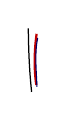
\begin{tikzpicture}[x=1em,y=1em,baseline=0pt]\draw[black,line width=.45pt] (.04,.2)..controls(.05,-.65)and(.08,-1.35)..(.16,-2.1);
\draw[red!75!black,line width=.8pt] (.34,0)..controls(.27,-.5)and(.23,-1.2)..(.33,-1.85);
\draw[blue!40!black,line width=.4pt] (.38,-.15)..controls(.25,-.7)and(.35,-1.55)..(.35,-1.92);\end{tikzpicture}}
\normalmarginpar
\[
\begingroup
\setbox0=\hbox{$\displaystyle\begin{array}{l}
\deleted{\unsure{\mathcal N_r(uv)|N_r(uv)}\leq\mathcal N_p(u)\mathcal N_q(v)}\\[.6ex]
\inserted{\|uv\|_r\leq\|u\|_p\|v\|_q}\quad\left(\frac1r=\frac1p+\frac1q\right)
\end{array}$}
\smash{\rlap{
\begin{tikzpicture}[x=\wd0,y=1ex,baseline=0pt]\draw[red!75!black,line width=1pt] (-.04,4.0)..controls(.18,3.8)and(.47,4.35)..(.72,4.3);
\draw[red!75!black,line width=1pt] (-.02,3.8)--(-.035,-3.2)..controls(.20,-3.4)and(.57,-2.9)..(1.05,-3.3);
\draw[red!75!black,line width=1.1pt] (1.02,2.5)..controls(1.05,1.4)and(1.02,-1.5)..(1.02,-3.2);
\draw[black,line width=.65pt] (.06,1.7)--(.045,.35)--(.20,3.25)--(.17,1.5)--(.30,3.8)--(.21,.1)--(.42,2.7)--(.36,.3)--(.50,2.35)--(.42,-.2)--(.58,1.25);
\draw[black,line width=.45pt] (-.04,-3.35)..controls(.27,-3.6)and(.66,-2.85)..(.96,-3.8);\end{tikzpicture}}}\box0
\endgroup
\]

\deleted{(\unsure{la somme} \illegible{3} \unsure{si tous les} \illegible{1})}

Le cas le plus important de l'inégalité (37) est celui où $s=1$, i.e. où $p$ et $q$ sont deux ``exposants conjugués''; \deleted{\unsure{Nous y reviendrons} \illegible{1}} \inserted{dans ce cas, (32) est d'ailleurs contenu dans} l'\deleted{\unsure{inégalité du|inégalités au} N\textsuperscript{o} suiv., en une formule plus frappante.}

\[
\begingroup
\setbox0=\hbox{$\displaystyle\|uv\|_1\leq\|u\|_p\|v\|_{p'}\quad\left(\frac1p+\frac1{p'}=1\right)$}
\begin{array}{ll}\textcircled{38}&\smash{\rlap{\begin{tikzpicture}[x=\wd0,y=1ex,baseline=0pt]\draw[red!75!black,line width=1pt] (.025,1.9)..controls(.27,2.3)and(.39,4.2)..(1.04,4.05);
\draw[red!75!black,line width=1pt] (-.025,1.75)--(-.05,-1.8)..controls(.25,-1.65)and(.58,.2)..(1.04,-.4);\end{tikzpicture}}}\box0\end{array}
\endgroup
\]

\deleted{(29) \unsure{qui est|si tous} : l'inégalité de Hölder \unsure{ordinaire}}. \inserted{(38) résulte d'ailleurs aussi de (32), grâce à l'inégalité de Hölder ordinaire}
\par\noindent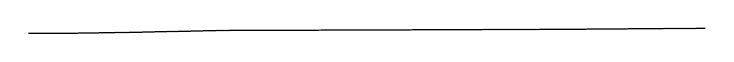
\begin{tikzpicture}[x=1cm,y=1ex,baseline=0pt]\draw[line width=.45pt] (0,0)..controls(.9,-.02)and(1.7,.15)..(2.6,.25)..controls(4.7,.28)and(6.6,.31)..(8.6,.42);\end{tikzpicture}

\reversemarginpar
\margin{\begin{tikzpicture}[x=1em,y=1em,baseline=0pt]\draw[line width=.5pt] (0,0)--(.5,.6);\end{tikzpicture}\par
Expliquer \unsure{l'itération|l'introduction} d'une \illegible{1}\par
\begin{tikzpicture}[x=1em,y=1em,baseline=0pt]\draw[line width=.55pt] (0,-.2)..controls(.65,.5)and(1.05,1.9)..(1.85,3.1);\end{tikzpicture}}
\normalmarginpar

\uline{Corollaire 4}. Soient $E,F,G$ trois espaces de Hilbert de $=$ dimension finie $n$, $u$ un op. cpt de $E$ dans $F$, $v$ un op. cpt de $F$ dans $G$, $f$ \inserted{$\unsure{(t_1,-t_n)|(s_1,-s_n)}$} une fonction \deleted{\unsure{sym.}} de $n$ arguments $t_i>0$ telle que $f(e^{t_{\unsure{i|1}}},-e^{t_n})$ soit fonction convexe de $(t_i)\in R^n$. Sous ces conditions, \inserted{si \deleted{\unsure{l'un de ces}} \inserted{$u$ et $v$} sont inversibles \unsure{ou|on a}} \deleted{la \unsure{formule}} \inserted{si $f$ est définie et continue pour $s_i\geq0$, on a}

\reversemarginpar
\margin{\textcolor{red!75!black}{\unsure{?}}\quad
\begin{tikzpicture}[x=1em,y=1em,baseline=0pt]\draw[red!75!black,line width=1.0pt] (0,.7)--(.12,-1.0);\end{tikzpicture}}
\normalmarginpar

\[
\begin{array}{ll}(39)&\displaystyle f(\rho_1(uv),-\rho_n(uv))\leq f(\rho_1(u)\rho_1(v),-\rho_{\unsure{n}}(u)
\end{array}
\]

En effet, \deleted{\unsure{on sait du}} \inserted{utilisant les conditions} du th. 1, 2\textsuperscript{o}, hyp. b),

\reversemarginpar
\margin{\uline{petits} \uline{caractères}}
\normalmarginpar

en vertu de

\[
\begin{array}{ll}(40)&\displaystyle\prod\rho_i(uv)=\deleted{f(uv)}\prod\rho_i(u)\rho_i(v)\end{array}
\]

\deleted{En effet,} \inserted{Pour vérifier (40),} on \deleted{\unsure{élève au carré}} \inserted{peut supposer} \deleted{est ramené} que $E=F=G$, alors les deux mb. de (35) sont resp\textsuperscript{t}. $|\det(uv)|$ et $|\det u|\,|\det v|$ (formule (\unsure{26|16})) d'où le résultat. Si $u$ et $v$ sont q.qcon\unsure{ques} mais $f$ définie et continue pour $t_i\geq0$, (39) sera encore valable par prolongement par continuité à partir du cas précédent.

Donner des liaisons sur la composition des opérateurs comme multiplication

\reversemarginpar\margin{93}\normalmarginpar

\cotefile{1}
\scanpage{93}

\uline{Th 4} (\uline{troisième th. de convexité dans les espaces de Hilbert})

\reversemarginpar
\margin{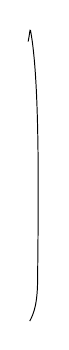
\begin{tikzpicture}[x=1cm,y=1cm]
\draw[line width=.35pt] (0,3.55)..controls (.02,3.64) and (.02,3.72)..(.03,3.69)..controls (.15,3.05) and (.13,1.55)..(.12,.54)..controls (.12,.22) and (.07,.09)..(.02,0);
\end{tikzpicture}}
\normalmarginpar
Soient $E,F$ deux espaces de Hilbert, $u,v$ deux opérateurs compacts de $E$ dans $F$, soit enfin $\varphi\inserted{(s_1,\mathord{-}s_n)}$ une fonction \deleted{\unsure{continue|convexe} symétrique}\inserted{convexe symétrique \unsure{croiss.|croissante} \deleted{et \unsure{épist.}}} de $n$ arguments $s_i\geq0$, \deleted{telle que $\unsure{f(e^{t_1},\quad e^{t_n})|f e^{t_1},\quad e^{t_n})}$ soit fonction convexe de $(\unsure{h|t_i})\in R^n$. Alors,}\inserted{Alors}

\[
\text{(41)}\qquad
\varphi(\rho_1(u+v),\mathord{-}\,\mathord{-},\rho_n(u+v))\leq
\varphi(\rho_1(u)+\rho_1(v),\mathord{\cdot}\,\mathord{-},\rho_n(u)+\rho_n(v))
\]

En effet, c'est un cas particulier du Th. 1, 1\uuline{°}, hypothèse c, compte tenu des formules du N\uline{°} 1.

\begingroup
\setbox0=\vbox{\hsize=\linewidth
\noindent\deleted{\uline{Corollaire} \unsure{Soit|Soient|Etant} $u$ et $v$ étant comme ci-dessus, soit $\varphi(s)$ une fonction convexe \inserted{\unsure{croiss.|croissante}} de $s\geq0$, alors on a pour tout entier $n>0$}
\[
\deleted{\text{(42)}\qquad\sum_1^n\varphi(\rho_i(u+v))\leq\sum_1^n\varphi(\rho_i(u)+\rho_i(v))}
\]}
\dimen0=\wd0\advance\dimen0 by4pt
\dimen2=\ht0\advance\dimen2 by-2pt
\dimen4=\dp0\advance\dimen4 by2pt
\dimen6=\ht0\advance\dimen6 by-12pt
\noindent\rlap{\begin{tikzpicture}[overlay,baseline=0pt]
\draw[line width=.35pt] (-3pt,\the\dimen2)..controls (-2pt,\the\dimen6) and (-3pt,4pt)..(0pt,-\the\dimen4)--(9pt,-\the\dimen4);
\draw[line width=.35pt] (\the\dimen0,\the\dimen6)..controls (\the\dimen0,12pt) and (\the\dimen0,4pt)..(\the\wd0,-\the\dimen4);
\end{tikzpicture}}\box0
\endgroup

Nous serons surtout \unsure{intéressé|intéressés} par le

\uline{Corollaire} 1 Soient \deleted{$u$ et $v$ comme ci-dessus,}\inserted{$E$ et $F$ deux espaces de Hilbert,} et soit $N$ \uline{une norme de Schatten} sur $R^n$, \deleted{alors la quantité} posons, pour \deleted{tout} opérateur compact $u$ de $E$ dans $F$

\[
\text{(4\unsure{3|2})}\qquad
\lVert u\rVert_N=N(\rho_1(u),\mathord{-}\rho_n(u))
\]

Alors on a

\begin{center}
\(\text{(44)}\qquad\)
\begingroup
\setbox0=\hbox{$\lVert u+v\rVert_N\leq\lVert u\rVert_N+\lVert v\rVert_N$}
\dimen0=\wd0\advance\dimen0 by6pt
\dimen2=\ht0\advance\dimen2 by5pt
\dimen4=\dp0\advance\dimen4 by4pt
\dimen6=\dimen2\advance\dimen6 by-3pt
\leavevmode\hspace{3pt}
\rlap{\raise\dimen2\hbox{$\deleted{\lVert\lambda u\rVert_N=|\lambda|\lVert u\rVert_N}$}}
\rlap{\begin{tikzpicture}[overlay,baseline=0pt]
\draw[red,line width=.8pt] (-3pt,\the\dimen2)--(\the\wd0,\the\dimen2)..controls (\the\dimen0,\the\dimen2) and (\the\dimen0,\the\dimen6)..(\the\wd0,1pt);
\draw[red,line width=.8pt] (-3pt,\the\dimen2)--(-3pt,-\the\dimen4)--(\the\wd0,-\the\dimen4)--(\the\wd0,-1pt);
\end{tikzpicture}}
\box0\hspace{6pt}
\endgroup
\end{center}

\deleted{et $\unsure{u\to\lVert u\rVert_N}$ \unsure{définit|est donc} \illegible{2} \unsure{$u\in L_0(E,F)$|$(L_0(E,F))$} \unsure{tels que|sous-espace} \unsure{Si} $N$ est une norme de \unsure{Schatten} \unsure{sur} $R\quad\unsure{R_+^{(n)}|R^{(N)}|R^{(\underline N)}}$}

En effet, $N(s_1,\mathord{-}s_n)$ pour $s_i\geq0$ satisfait aux conditions de (41), on a donc

\[
N(\rho_1(u+v),\mathord{-},\rho_i(u+v))\leq
N(\rho_1(u)+\rho_1(v),\mathord{\cdot}\,\mathord{-},\rho_i(u)+\rho_i(v))
\]

et le second \unsure{$=$b|$\bar m$b} est majoré par $N(\rho_1(u),\mathord{-},\rho_n(u))+N(\rho_1(v),\mathord{-},\rho_n(v))$ puisque $N$ est une norme, d'où (44).

En particulier

\uline{Corollaire 1} \deleted{\unsure{Pour les|Soient}} si $u,v\in L_0^{\unsure{p}}(E,F)$, \deleted{\unsure{alors|et si}} \unsure{cf|(f} $1\leq p\leq+\infty$)) $\mathord{\cdot}\,\mathord{-}\,.$ pour \deleted{\unsure{tout}} \inserted{entier $n>0$}

\[
\deleted{\lVert u+v\rVert_p\leq}
\]
\[
\text{(45)}\qquad
\left(\sum_1^n(\rho_i(u+v))^p\right)^{1/p}\leq
\left(\sum_1^n\rho_i(u)^p\right)^{1/p}+
\left(\sum_1^n\rho_i(v)^p\right)^{1/p}
\]

donc \unsure{par|en} \deleted{\unsure{$(N$|$(\varphi$|(passant|(passage} \illegible{3}} \deleted{$\unsure{\sum}$}

\begin{center}
\(\text{(46)}\qquad\)
\begingroup
\setbox0=\hbox{$\lVert u+v\rVert_p\leq\lVert u\rVert_p+\lVert v\rVert_p$}
\dimen0=\wd0\advance\dimen0 by7pt
\dimen2=\ht0\advance\dimen2 by5pt
\dimen4=\dp0\advance\dimen4 by3pt
\dimen6=\dimen2\advance\dimen6 by2pt
\dimen8=\dimen0\advance\dimen8 by12pt
\leavevmode\hspace{3pt}
\rlap{\begin{tikzpicture}[overlay,baseline=0pt]
\draw[red,line width=.5pt] (-13pt,\the\dimen6)--(\the\dimen8,\the\dimen6);
\draw[red,line width=.5pt] (-3pt,\the\dimen2)--(-3pt,-\the\dimen4)--(\the\dimen0,-\the\dimen4)--(\the\dimen0,\the\dimen2);
\end{tikzpicture}}
\box0\hspace{7pt}
\endgroup
\end{center}

\reversemarginpar
\margin{94}
\normalmarginpar

\scanpage{94}

\textcircled{5.} \uline{Classes remarquables d'opérateurs dans l'espace de Hilbert}

Nous commençons par donner un {\color{red}\uline{\color{black}exposé}} de la théorie de Schatten, \deleted{\unsure{qui est|que nous}} sous une forme simplifiée rendue possible par la \deleted{\unsure{lemme}}\inserted{méthode du \unsure{minimum|minimax}} de Weyl, et en {\color{red}\uline{\color{black}y apportant}} q.q \unsure{petits|menus} compléments.

{\reversemarginpar\margin{{\color{red}?}}}

\deleted{\unsure{Déf}} Rappelons la

{\reversemarginpar\margin{\begin{tikzpicture}[baseline=(current bounding box.north)]\draw[line width=.4pt] (0,0) .. controls (.04,-.8) and (.02,-1.7) .. (.03,-2.7) .. controls (.03,-3.2) and (.07,-3.4) .. (.13,-3.5) .. controls (.10,-4.3) and (.12,-5.5) .. (.08,-6.5);\end{tikzpicture}}}
\uline{Définition 1} \deleted{Soit} Une norme $N$ sur $R^n$ est dite \uline{norme de Schatten} si elle est symétrique, satisfait à

\deleted{\unsure{à|2|3}}

\[
\begin{array}{@{}l@{\qquad}l@{}}
(1)&\displaystyle N(x_1,\mathord{-}x_n)=N(|x_1|,\mathord{-}|x_n|)
\end{array}
\]

\deleted{et si elle} \unsure{si|2.} elle est croissante \deleted{\unsure{sur l'ensem}} sur l'ens. des $x_i\geq 0$, et \deleted{\unsure{est satisf}} est normalisée par $N(1,0,\mathord{-}0)=1$

Une norme $N$ sur $R^{(\underline N)}$ \deleted{$\unsure{R}\underline N$ \unsure{ensemble|espace des}} (\unsure{espace|anneau} des suites infinies \deleted{\unsure{finies}} nulles sauf un nb fini de termes) est appellée une norme de Schatten, si \inserted{pour tout entier $n>0$,} elle induit \deleted{sur} de sur $R^n$ une norme de Schatten

($R^n$ sera ici identifié \deleted{\unsure{à l'espace des suites}}\inserted{au sous-espace} de $R^{(\underline N)}$ formé des suites nulles à partir du rang $n+1$). Notons qu'une norme de Schatten sur $R^n$ induit sur $R^m$ ($m\leq n$) une norme de Schatten. \deleted{\unsure{Tout cette théorie résulte que|Il est immédiat que}}\inserted{Exemples de normes de} Schatten\,:

\deleted{\unsure{Supposons|l'app.}}

\[
\deleted{N_p(\{x_i\})\unsure{=}\left(\sum |x_i|^p\right)^{1/p}\quad\text{\unsure{où }}1\leq p}
\]

les normes $N_p((x_i))=\lVert(x_i)\rVert_p$, définies \unsure{par|pour} \deleted{$1\leq p\leq\unsure{+\infty|\infty}$ \unsure{par}}

{\reversemarginpar\margin{\begin{tikzpicture}[baseline=(current bounding box.north)]\draw[line width=.5pt] (0,0)--(.12,-.22);\end{tikzpicture}}}
\[
\begin{array}{@{}l@{\qquad}l@{}}
(2)&\displaystyle \lVert(x_i)\rVert_p=\left(\sum |x_i|^p\right)^{1/p}\qquad (1\leq p<+\infty)
\end{array}
\]

\[
\begin{array}{@{}l@{\qquad}l@{}}
\deleted{\unsure{4}}\ (3)&\displaystyle \lVert(x_i)\rVert_\infty=\underset{i}{\operatorname{Sup}}\,|x_i|
\end{array}
\]

{\reversemarginpar\margin{\begin{tikzpicture}[baseline=(current bounding box.north)]\draw[line width=.4pt] (-.5,-.12) .. controls (-.6,0) and (-.2,0) .. (0,0) .. controls (.08,-.05) and (.04,-.5) .. (.01,-1.2) .. controls (0,-2.4) and (-.2,-3.4) .. (-.45,-4.2);\end{tikzpicture}}}
Si $N_0$ est une norme de Schatten \deleted{alors} sur $R^n$, il existe toujours une norme de Schatten $N$ sur $R^{(\underline N)}$ \deleted{\unsure{qui}}
{\reversemarginpar\margin{{\color{red}?}}}
{\color{red}\uline{\color{black}induise}} $N_0$\deleted{, \unsure{p. ex.,} \illegible{1}} si, pour \deleted{\unsure{toute|tout}} $x=(x_i)\in\underline{C}_0$, on désigne par
{\reversemarginpar\margin{{\color{red}?}}}
$(\unsure{\rho|R|f}_i(x))$ la suite des $|x_i|$ \deleted{{\color{red}\uline{\color{black}\unsure{rangés|arrangés}}}}\inserted{non nuls}
{\color{red}\uline{\color{black}rangés par ordre de grandeur décro}}issant, on peut p. ex. poser $N(x)=N_0(\rho_1(x),\mathord{-}\rho_n(x))$. Il est trivial

{\reversemarginpar\margin{95}}

\scanpage{95}

\reversemarginpar
\margin{\begin{tikzpicture}[x=1cm,y=1cm,baseline=(current bounding box.north)]
\draw[line width=.25pt] (.04,0) .. controls (.00,-.20) and (.03,-1.1) .. (.10,-2.4) .. controls (.17,-3.6) and (.31,-5.2) .. (.28,-5.73);
\draw[line width=.25pt] (.28,-5.79) .. controls (.10,-5.81) and (-.05,-5.96) .. (-.24,-6.13);
\end{tikzpicture}}
\normalmarginpar

que $N(x)$ induit sur $R^n$ la fonction $N_0(x)$, et qu'on a $N(\lambda x)=|\lambda|N(x)$ et $N(x)=0\Rightarrow x=0$, il faut seulement prouver $N(x+y)\leq N(x)+N(y)$ (\textcolor{red}{\uline{\textcolor{black}{est}}} valable $=$ pour $x,y\in c_0$.) Pour ceci, on \deleted{\unsure{regarde} $(x_i)$ et $(y_i)$ comme \unsure{les}}\inserted{remarque que si} $u_x$ est l'opération de multiplication par $x$ dans $\ell^2$ (qui est un opérateur cpt pour $x\in c_0$), on a \deleted{$u_{x+y}=u_x$} $\rho_i(u_x)=\rho_i(x)$, d'autre part \deleted{\unsure{que|$\rho_i$}} $u_{x+y}=u_x+u_y$, et l'inégalité à prouver résulte alors du N\textsuperscript{\uline{o}}~4, th.~4, corollaire. En $=$ temps, les normes \deleted{\unsure{ft}}\inserted{de Schatten} ainsi associées à des normes \deleted{\unsure{de}} de Schatten $N_0$ sur $R^n$ \deleted{donnent} démontrent qu'il existe une infinité \inserted{continue} de normes de Schatten sur $R^{(\underline N)}$ équivalentes à la norme induite par $c_0$.

Soit $N$ \deleted{\unsure{est}} une norme de Schatten sur \deleted{$\unsure{R^I|R^n}$ \unsure{finies|fini}} $R^{(\underline N)}$. \deleted{Soit $\unsure{\ell_N}$ $\ell^N$ \unsure{l'espace des}}\inserted{Pour \deleted{toute}} suite \deleted{\unsure{réelle}} complexe $x=(x_i)$ \deleted{telle que \unsure{la suit}} \deleted{\unsure{on pose|$N\quad\rho$}} \deleted{soit $\unsure{N(x\mathord{-}x|N(x\,x}$}

\[
\deleted{N(|x_1|,\mathord{\cdot}\,\mathord{-}|x_n|,0,0,\mathord{-}\,\mathord{-}\,\mathord{\cdot})\quad\text{croît avec }n,\quad\text{on pose.}}
\]

Soit $|x|_n=(|x_1|,\mathord{\cdot}\,\mathord{-}|x_n|,0,\mathord{-}\,\mathord{-}0)$. \deleted{\unsure{On a aussitôt|Comme on a}}\inserted{Si $n$ varie} \deleted{alors $|x+y|_n\leq |x|_n+|y|_n$} $|x|_n$ est une suite croissante d'éléments positifs de $R^{(N)}$, posons

\[
\text{(4)}\qquad N(x)=\lim_n N(|x|_n)
\]

\inserted{c'est un nb $\geq 0$ fini ou infini} La valeur \deleted{\unsure{impropre|infinie|ainsi} \unsure{est définie|désignée}} de $N(x)$, qui coïncide avec \deleted{\unsure{$N(x)$|celle}} \inserted{quand $x\in R^{(N)}$.} On a

\[
\text{(5)}\qquad N(\lambda x)=|\lambda|N(x),\qquad N(u+y)\leq N(\unsure{u|x})-N(y)
\]

\deleted{si $N(x)<+\infty$} \inserted{et dans} la première formule, \deleted{\unsure{il est à dire|étant dit} que \unsure{son deuxième mb a un sens}, i.e $|\lambda|$} \inserted{il faut prendre au deuxième}
\reversemarginpar
\margin{\textcolor{red}{?}}
\normalmarginpar
mb la valeur \textcolor{red}{\uline{\textcolor{black}{zéro}}} s'il \deleted{\unsure{est sous}}\inserted{se présente sous la} forme indéterminée $0\times\infty$. La deuxième formule résulte de ce que \deleted{$N(x$} $|x+y|_n\leq |x|_n+|y|_n$, d'où $N(|x+y|_n)\leq N(|x|_n+|y|_n)\leq N(|x|_n)+N(|y|_n)$.

\deleted{Soit} Soit $\ell^N$ l'espace des suites complexes $x$ telles que $N(x)<\infty$, espace \unsure{contenant|vectoriel} au moins \deleted{\unsure{$C^{(N)}$|celles}} les suites complexes nulles à partir \deleted{\unsure{de rang|de mult}} d'un certain rang. \unsure{Sur|Par|Pour} $(5)$, on voit que $N(x)$ est une \uline{norme} sur $\ell^N$.

\deleted{\unsure{De plus|D'ailleurs}, $\ell^N$ est \unsure{un espace de} \illegible{2} \unsure{positivité}. D'où \unsure{les inj} $R^{(N)}\subset\ell^N$, et $N(x)$ induit \unsure{par hypothèse}, \unsure{donc} ($=$ \illegible{1} $\unsure{\alpha^i|\alpha^{(i)}}$), est \illegible{2} \unsure{le candidat|la convergence} dans $\ell^N$, \unsure{elles coïncident donc forcément|la convergence en chaque point}}

\reversemarginpar
\margin{96}
\normalmarginpar

\cotefile{1}
\scanpage{96}

\deleted{\unsure{On a, si} $N\unsure{<|\leq}$}

\[
\begin{array}{@{}l@{\qquad}l@{}}
\deleted{(6)} & \deleted{\ell^1\subset\ell^N\subset\ell^\infty}
\end{array}
\]

\deleted{et la norme de $\ell^1$ est plus fine que celle induite par $\ell^N$, \deleted{\unsure{qui est}} et la norme de $\ell^N$ est moins fine que celle induite par}

Si $N_{\deleted{\unsure{1}}}^{\inserted{'}}$ et $N_{\deleted{\unsure{2}}}^{\inserted{''}}$ sont deux normes de Schatten telles que $N_{\deleted{1}}^{\inserted{'}}\leq N_{\deleted{2}}^{\inserted{''}}$, il est immédiat qu'on a $\ell^{N_{\deleted{1}}^{\inserted{'}}}\subset\ell^{N_{\deleted{2}}^{\inserted{''}}}$, et la norme de $\ell^{N'}$ \deleted{$\unsure{\ell^{N_1}\subset\ell^{N_2}|\ell^{N'}\subset\ell^{N''}}$} est plus fine que celle induite par $\ell^{N''}$.

\deleted{En particulier,} En particulier, si on remarque que toute norme de Schatten est comprise entre les normes de Schatten $N_1(x)=\sum_i |x_i|$ et $N_\infty(x)=\underset{i}{\operatorname{Sup}}\,|x_i|$, et que les espaces $\ell^N$ associés à ces dernières sont \deleted{$\unsure{\ell^1|\ell^{N_1}}$ et $\unsure{\ell^N|\ell^{N_\infty}}$} $\ell^1$ et $\ell^\infty$, \deleted{\unsure{est|et}} on voit que

\[
\begin{array}{@{}l@{\qquad}l@{}}
(6) & \ell^1\subset\ell^N\subset\ell^\infty
\end{array}
\]

les applications identiques \deleted{\unsure{de $\ell^1$}} $\ell^1\to\ell^N$ et $\ell^N\to\ell^\infty$ étant de norme $\leq 1$.

\deleted{Notons la formule}

\[
\begin{array}{@{}l@{\qquad}l@{}}
\deleted{(7)} & \deleted{\deleted{\sum}\quad N\left(\sum_n x_{\unsure{i}}^{k}\right)\leq\sum_k N(x^k)}
\end{array}
\]

\reversemarginpar\margin{\rotatebox{25}{\unsure{Si Si|hi hi}}}\normalmarginpar
\deleted{valable pour toute suite $\deleted{\unsure{x^i=(x^i)|x^i=(x_i^i)|x^i=(x_j^i)}}$ de suites $x^k\in\unsure{C|\ell}^N$, qui soit \deleted{\unsure{convergente}} sommable pour chaque coordonnée $i$\,: $\sum_k|x_i^k|<+\infty$. Il suffit de prouver (7) si le \unsure{dernier|deuxième} mb est fini alors en posant $x=\sum_k x^k$, on aura $|x|_m\leq\sum_k|x^k|_m$ d'où $N(|x|_m)\leq N(\sum_k|x^k|_m)$}

\deleted{or \inserted{$N$ étant une fonction continue sur $R^m$, on aura.} $N(\sum_k|x^k|_m)\leq\lim_{\unsure{n|k}\to\infty}N(\sum_{k=1}^n|x^k|_m)$}

\deleted{et comme $N(\sum_{k=1}^{n}|x^k|_m)\leq\sum_{k=1}^n N(|x^k|_m)\leq\sum_{k=1}^{\unsure{\infty|n}} N(x^k)$, on aura $N(\sum_k|x^k|_m)\leq\sum_k N(x^k)$, donc pour tout $m$ on a $N(|x|_m)\leq\sum_k N(x^k)$, d'où par définition de $N(|x|)$ l'inégalité (7).}

\reversemarginpar\margin{97}\normalmarginpar

\scanpage{97}

On conclut de (7) que $\ell^N$ est \uline{complet}. Il suffit de prouver que \deleted{\unsure{toute}} \unsure{\deleted{suite}|suite} $(x^k)$ \deleted{dans $\ell^N$} d'éléments $x^k\in\ell^N$, telle que $\sum\lVert x^{k}\rVert_N<+\infty$, est sommable dans $\ell^N$. Or \deleted{elle} on aura \unsure{à|:} fortiori $\sum\lVert x^k\rVert_\infty<+\infty$, donc la \deleted{série} suite sera sommable dans $\ell^\infty$, \inserted{vers un $x\in\ell^\infty$} d'autre part on \deleted{\unsure{aura|aussi}} voit sur (7) que $x\in\ell^N$. D'autre part,

{\reversemarginpar\margin{Inutile, il suffit de procéder par dualité : $\ell^N$ est le dual de $\ell_N$.}}

on a

\[
N\left(x-\sum_{k=1}^n x^k\right)=\deleted{\unsure{\leq|\Rightarrow}}N\left(\deleted{\unsure{x-|x}}\sum_{n+1}^\infty x^k\right)\leq\sum_{n\unsure{-|+}1}^{\unsure{n|\infty}}N(x^k),
\]

qui tend vers \deleted{\unsure{l'$\infty$|zéro} \unsure{puisque la|pour}}\inserted{$0$ pour $n\to+\infty$}, puisque $\sum N(x^k)$ est une série convergente. Il s'ensuit que l'on a aussi $\sum x^k=x$ \uline{dans $\ell^N$}.

Soit $\ell_N$ l'adhérence de $C^{(\underline N)}$ dans $\ell^N$, comme $\ell^N$ est complet, $\ell_N$ s'identifie au complété de $C^{(\underline N)}$ pour la norme $N$. Il est encore trivial que si $N'\leq N''$, alors $\ell_{N'}\subset\ell_{N''}$, et \unsure{l'injection|l'application} identique $\ell_{N'}\to\ell_{N''}$ est de norme $\leq 1$. En particulier, les espaces $\ell_N$ associés à $N_1$ et $N_\infty$ étant resp. $\ell^1$ et $c_0$, on obtient

\[
\begin{array}{@{}l@{\qquad}l@{}}
(8)&\displaystyle \ell^1\subset\ell_N\subset c_0
\end{array}
\]

{\reversemarginpar\margin{\begin{tikzpicture}[x=0.13mm,y=-0.13mm,line cap=round,line join=round]
\draw[blue!60!black,line width=0.35mm] (12,25)--(25,27)--(37,28)--(54,28)--(69,29)--(81,31)--(94,31);
\draw[blue!60!black,line width=0.3mm] (32,28)--(48,27)--(64,28)--(78,26);
\draw[blue!60!black,line width=0.3mm] (32,31)--(45,30)--(60,31)--(74,31)--(87,32);
\end{tikzpicture}}}

\uline{Proposition} On a $\ell^N\subset c_0$ sauf si $N$ est équivalente \unsure{à|:} $N_\infty$.

\deleted{Notons la formule, qui précise la \unsure{condition|propriétés} \unsure{ci-dessus|suivantes}}

\[
\begin{array}{@{}l@{\qquad}l@{}}
\deleted{(9)}&\displaystyle \deleted{\underline{\ell}_N=\underline{\ell}^N\cap\underline{c}_0}
\end{array}
\]

\deleted{Il suffit de prouver que $x\in\ell^N\cap c_0$ implique $x\in\ell_N$. \unsure{Et} En effet, on aura}\raisebox{-0.8ex}[0pt][0pt]{\makebox[0pt][r]{\begin{tikzpicture}[x=0.15cm,y=0.15cm,baseline]
\draw[line width=0.45pt] (0,0)--(0.6,0);
\fill (1.3,0) circle (0.06);
\fill (2.3,-0.02) circle (0.07);
\draw[line width=0.45pt] (3.15,-0.02)--(3.75,-0.02);
\fill (4.2,-0.02) circle (0.07);
\draw[line width=0.45pt] (5.1,-0.02)--(5.8,-0.04);
\draw[line width=0.45pt] (6.75,-0.08)--(7.65,-0.08);
\fill (8.65,-0.1) circle (0.07);
\draw[line width=0.45pt] (9.6,-0.08)--(10.2,-0.08);
\end{tikzpicture}}}

Notons que $R^{(N)}$ est en dualité avec lui-$=$ par l'accouplement $\langle x,y\rangle=\sum x_i y_i$. Cela permet de faire correspondre à \deleted{toute} une norme $N$ sur $R^{(N)}$, la \uline{norme polaire}, notée $N'$, définie par

\[
\begin{array}{@{}l@{\qquad}l@{}}
(9)&\displaystyle N^\circ(y')=\underset{N(\unsure{y|x})\leq 1}{\operatorname{Sup}}\,|\langle x,y'\rangle|
\end{array}
\]

{\reversemarginpar\margin{De plus, \unsure{alors|clairement} \unsure{on a} $(N^\circ)^\circ=N$, on peut le vérifier .... \deleted{\unsure{on est ramené} \unsure{à|au|de} \illegible{1}}}}

Si $N$ est une norme de Schatten, on vérifie
{\reversemarginpar\margin{\begin{tikzpicture}[x=0.13mm,y=-0.13mm,line cap=round,line join=round]
\draw[line width=0.6mm] (45,21) .. controls (43,28) and (35,33) .. (37,45) .. controls (40,69) and (47,81) .. (71,92) .. controls (95,103) and (120,108) .. (140,104);
\draw[line width=0.6mm] (125,111) .. controls (91,126) and (50,148) .. (23,178) .. controls (18,184) and (19,186) .. (24,189);
\end{tikzpicture}}}
trivialement que $N^\circ$ est une norme de Schatten, et On \unsure{dira|dit} que \deleted{le dual de $\ell_N$ s'identifie à $\ell^{N'}$, l'accou\unsure{p|pl} \unsure{étant|ment} $\sum x_i x_i'$ est \unsure{abs\textsuperscript{t}} sommable, et que} \inserted{si $u\in\ell_N$, $u'\in\ell^{N^\circ}$, alors \deleted{\unsure{on a le}}}

{\reversemarginpar\margin{98}}
